\documentclass{beamer}	
\mode<presentation>
 
\usepackage{pdfpages}
\usepackage{fancyvrb}
\usepackage{chemarr}

\usepackage{amsmath}		%% mathematics typesetting
\usepackage{amssymb}
 
\usepackage{listings}   %% code listings

\usepackage{hyperref}

\usepackage{booktabs}

\usepackage{CJKutf8} %% typeset Chinese characters

\usepackage{pdfpages}

% Color and Theme. Can be changed. However, this one's quite nice.
\usetheme{Madrid}
\definecolor{theme}{rgb}{0.84,0,0.21}
\usecolortheme[named=theme]{structure}



%%  Title information
\title[M11.13.4 Nozizeption und Schmerz]{M11.13.4 Nozizeption und Schmerz}
\author[melanie.stefan@medicalschool-berlin.de]{}
\institute[]{Prof. Melanie Stefan \\ melanie.stefan@medicalschool-berlin.de}
\date{WiSe 2023/24}
 

% Table of contents to pop up at the beginning of each section
\AtBeginSection[]
{
  \begin{frame}<beamer>
    \frametitle{Outline}
    \tableofcontents[currentsection,currentsubsection]
  \end{frame}
}
 
\beamertemplatenavigationsymbolsempty

\begin{document}


{ \usebackgroundtemplate{
\includegraphics[width=1.2\paperwidth]{MSB_Titelseite.pdf}} 
\begin{frame}

 \maketitle 

$\,$\\[6cm] 


\end{frame} 
}


{ \usebackgroundtemplate{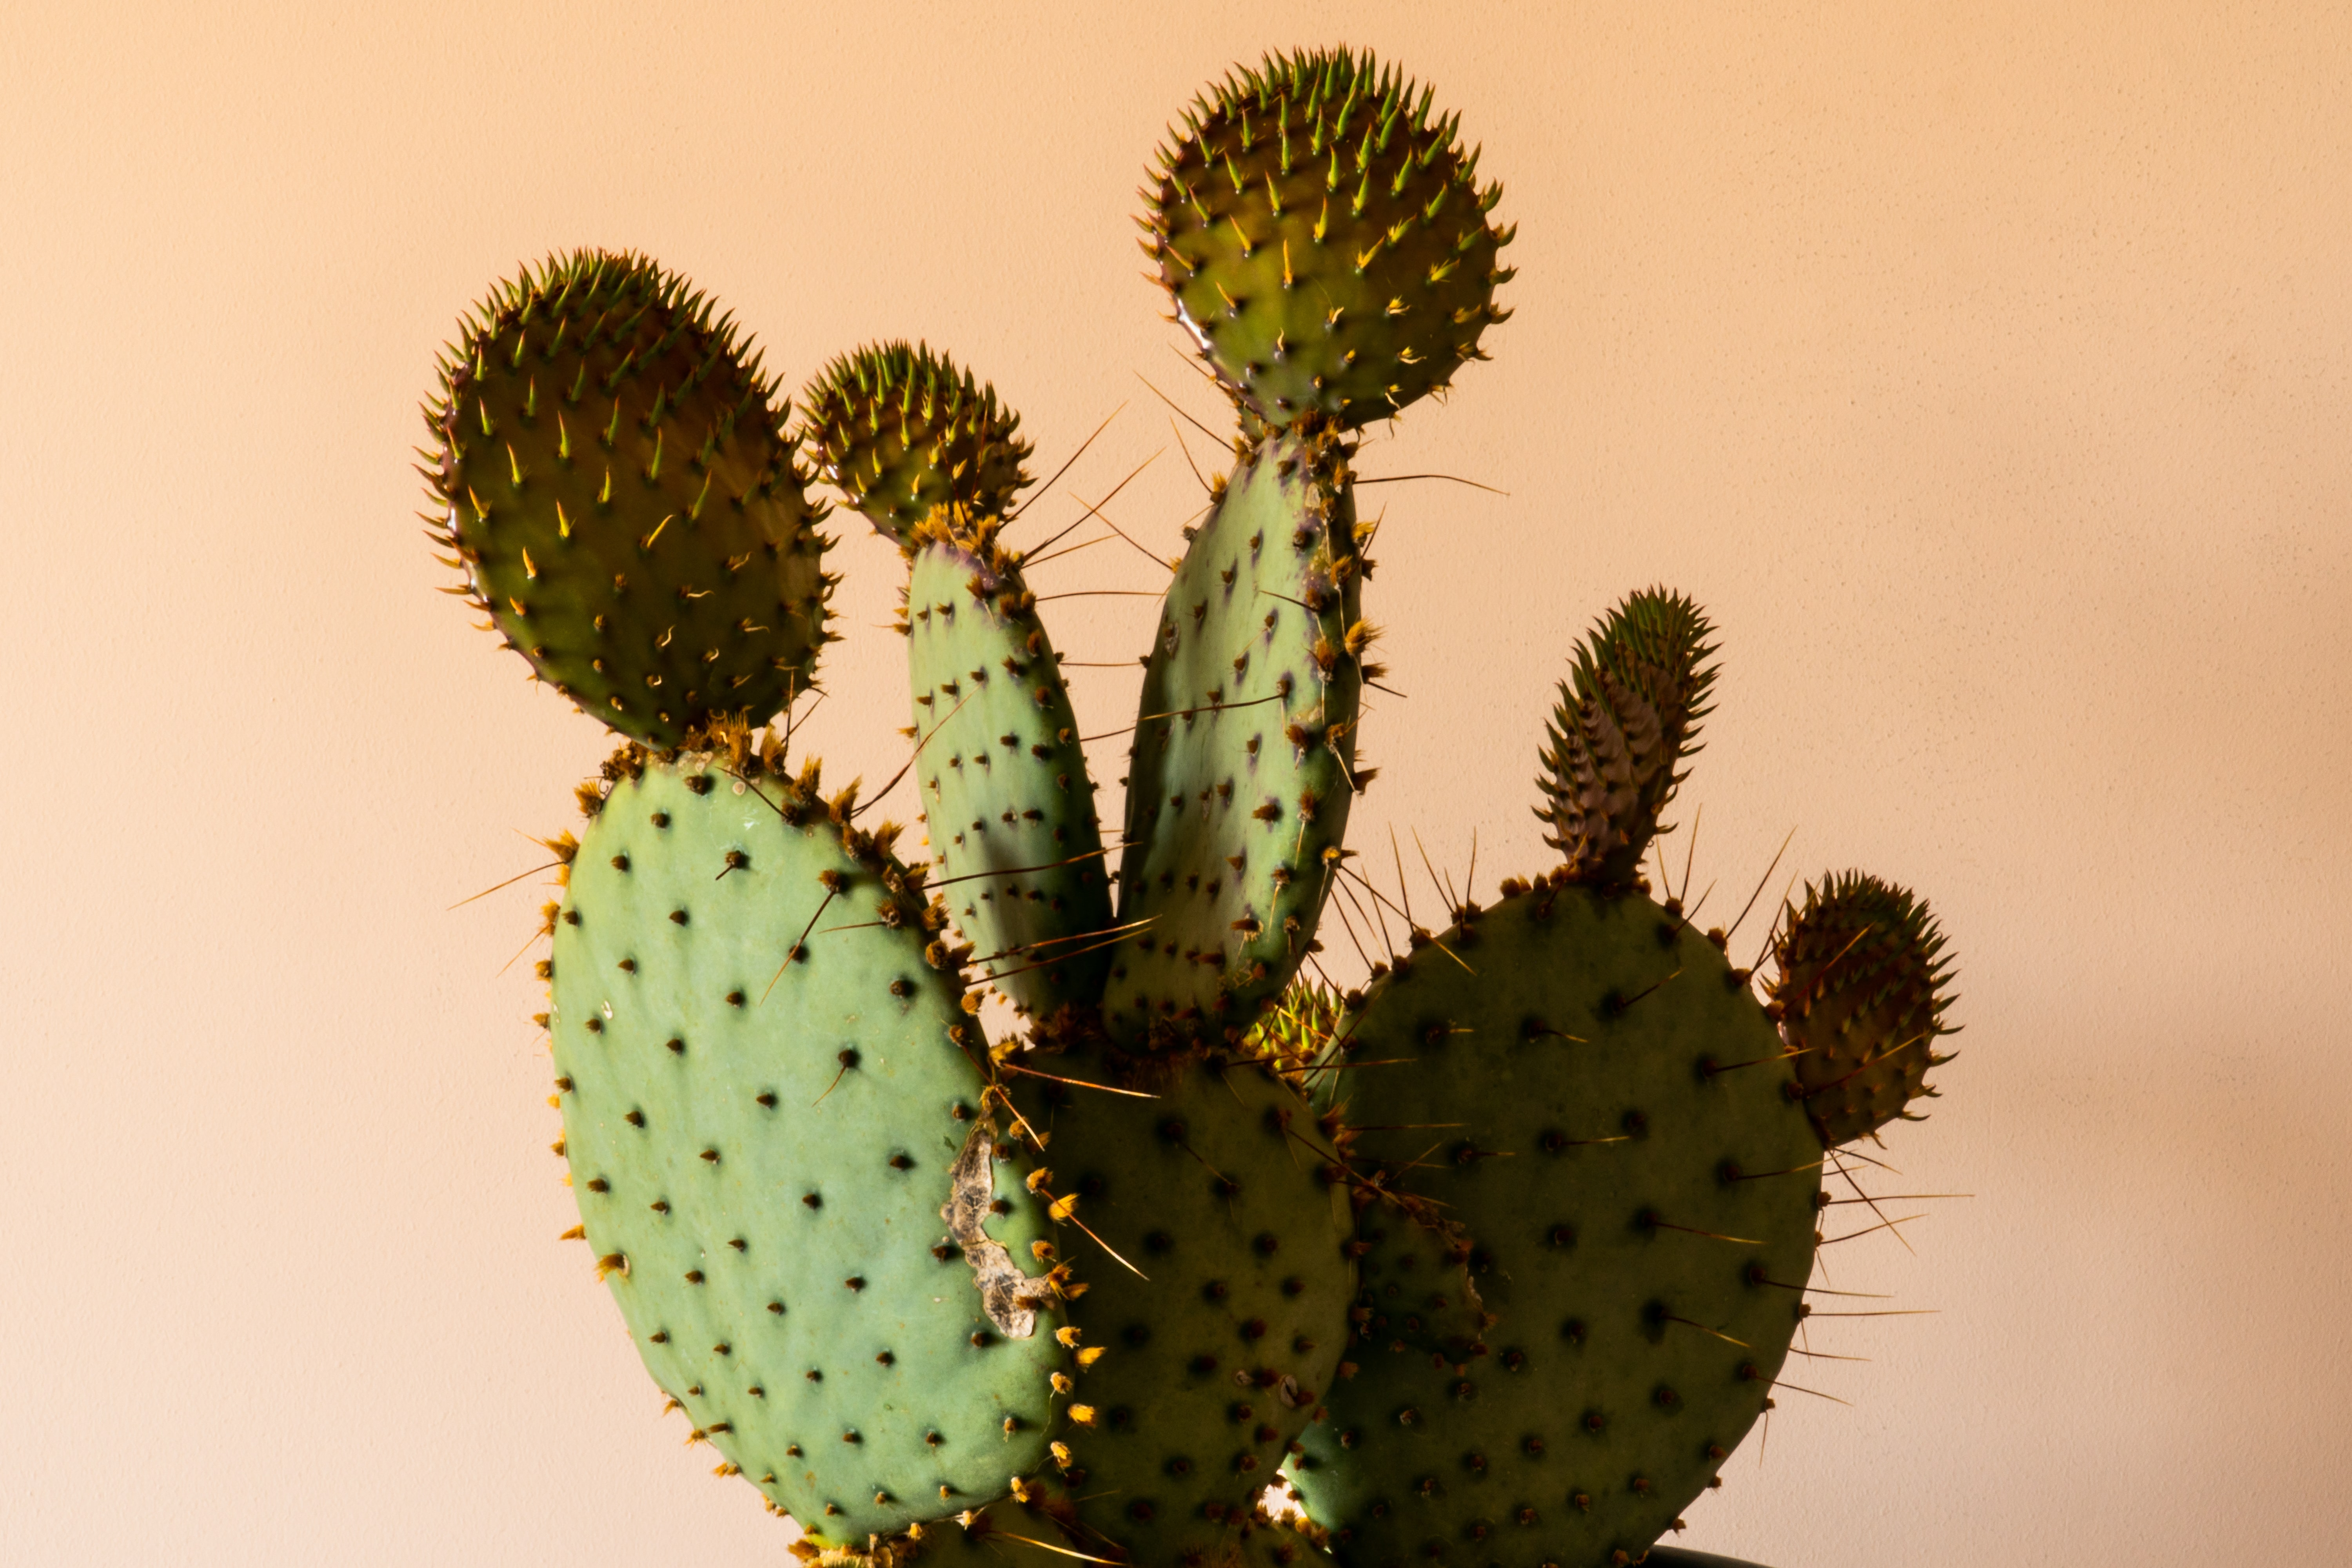
\includegraphics[width=1.2\paperwidth]{cactus.jpg}} 
\begin{frame}
\frametitle{Was wollten Sie schon immer über Schmerz wissen?}

\end{frame} 
}



%% Hook: 
\begin{frame}
\frametitle{Häufig gestellte Fragen zum Thema Schmerz}


\begin{itemize}
\item
Warum ist auf Sonnenbrand alles schmerzhaft, sogar ein T-Shirt?
\item
Wie funktioniert eigentlich Aspirin? 
\item
Warum können Schmerzen im Arm ein Anzeichen von Herzinfarkt sein? 
\item
Warum tut es weh, besonders scharfe Chilis zu essen?
\item
Warum kann man bei Schmerzen schlecht schlafen? 
\item
Warum haben manche Menschen nie Schmerzen? Und andere dauernd?
\item
Wie funktionieren Phantomschmerzen?  
\item
\dots 
\end{itemize}


\end{frame}




%% TLIA

\begin{frame}
\frametitle{In dieser Vorlesung geht es um die Schmerzwahrnehmung}
\begin{center}
\includegraphics[width=0.5\textwidth]{Schmerz_aufsteigend.png}
\end{center}

\end{frame}



%% Lernziele

\begin{frame}


 \frametitle{Nach dieser Vorlesung sollten Sie folgendes können}



\begin{block}{Grundlagen:}




\begin{itemize}

    \item 
Arten von Nozizeptoren beschreiben und erklären  %% 
    \item 
 schnellen und langsamen Schmerz unterscheiden und deren neurobiologische Grundlagen erläutern %%
    \item 
 endogene Mediatoren der Nozizeptorerregung benennen und erläutern %
    \item 
Hyperalgesie und Allodynie definieren %%
    \item 
 Neuropeptide beschreiben, die aus Nozizeptoren freigesetzt werden und deren Wirkung erläutern %% 
    \item 
 neurogene Vasodilatation und Entzündung erläutern
    \item 
 Aufsteigende Schmerzbahnen beschreiben %%
    \item 
 die Schmerzübertragung bei viszeraler Nozizeption erklären  %%
    \item 
erklären, welche  Hirnregionen an der Schmerzempfindung teilhaben %%
    \item 
 projizierten Schmerz definieren %%

\end{itemize}


\end{block}

\end{frame}


\begin{frame}


%% Lernziele
 \frametitle{Nach dieser Vorlesung sollten Sie folgendes können}
 

\begin{block}{Klinik:}

\begin{itemize}
    
\item 
Schmerztherapien aufzählen und erklären % 
    \item 
 Phantomschmerzen definieren% 
    \item 
 Beispiele für Krankheiten mit erhöhtem und vermindertem Schmerzempfinden geben. % 
\item
Head-Zonen beschreiben %
\end{itemize}


\end{block}



\end{frame}


%%% Main Body


\begin{frame}{Erinnerung: Wahrnehmungsbahn}
    
    \begin{center}
        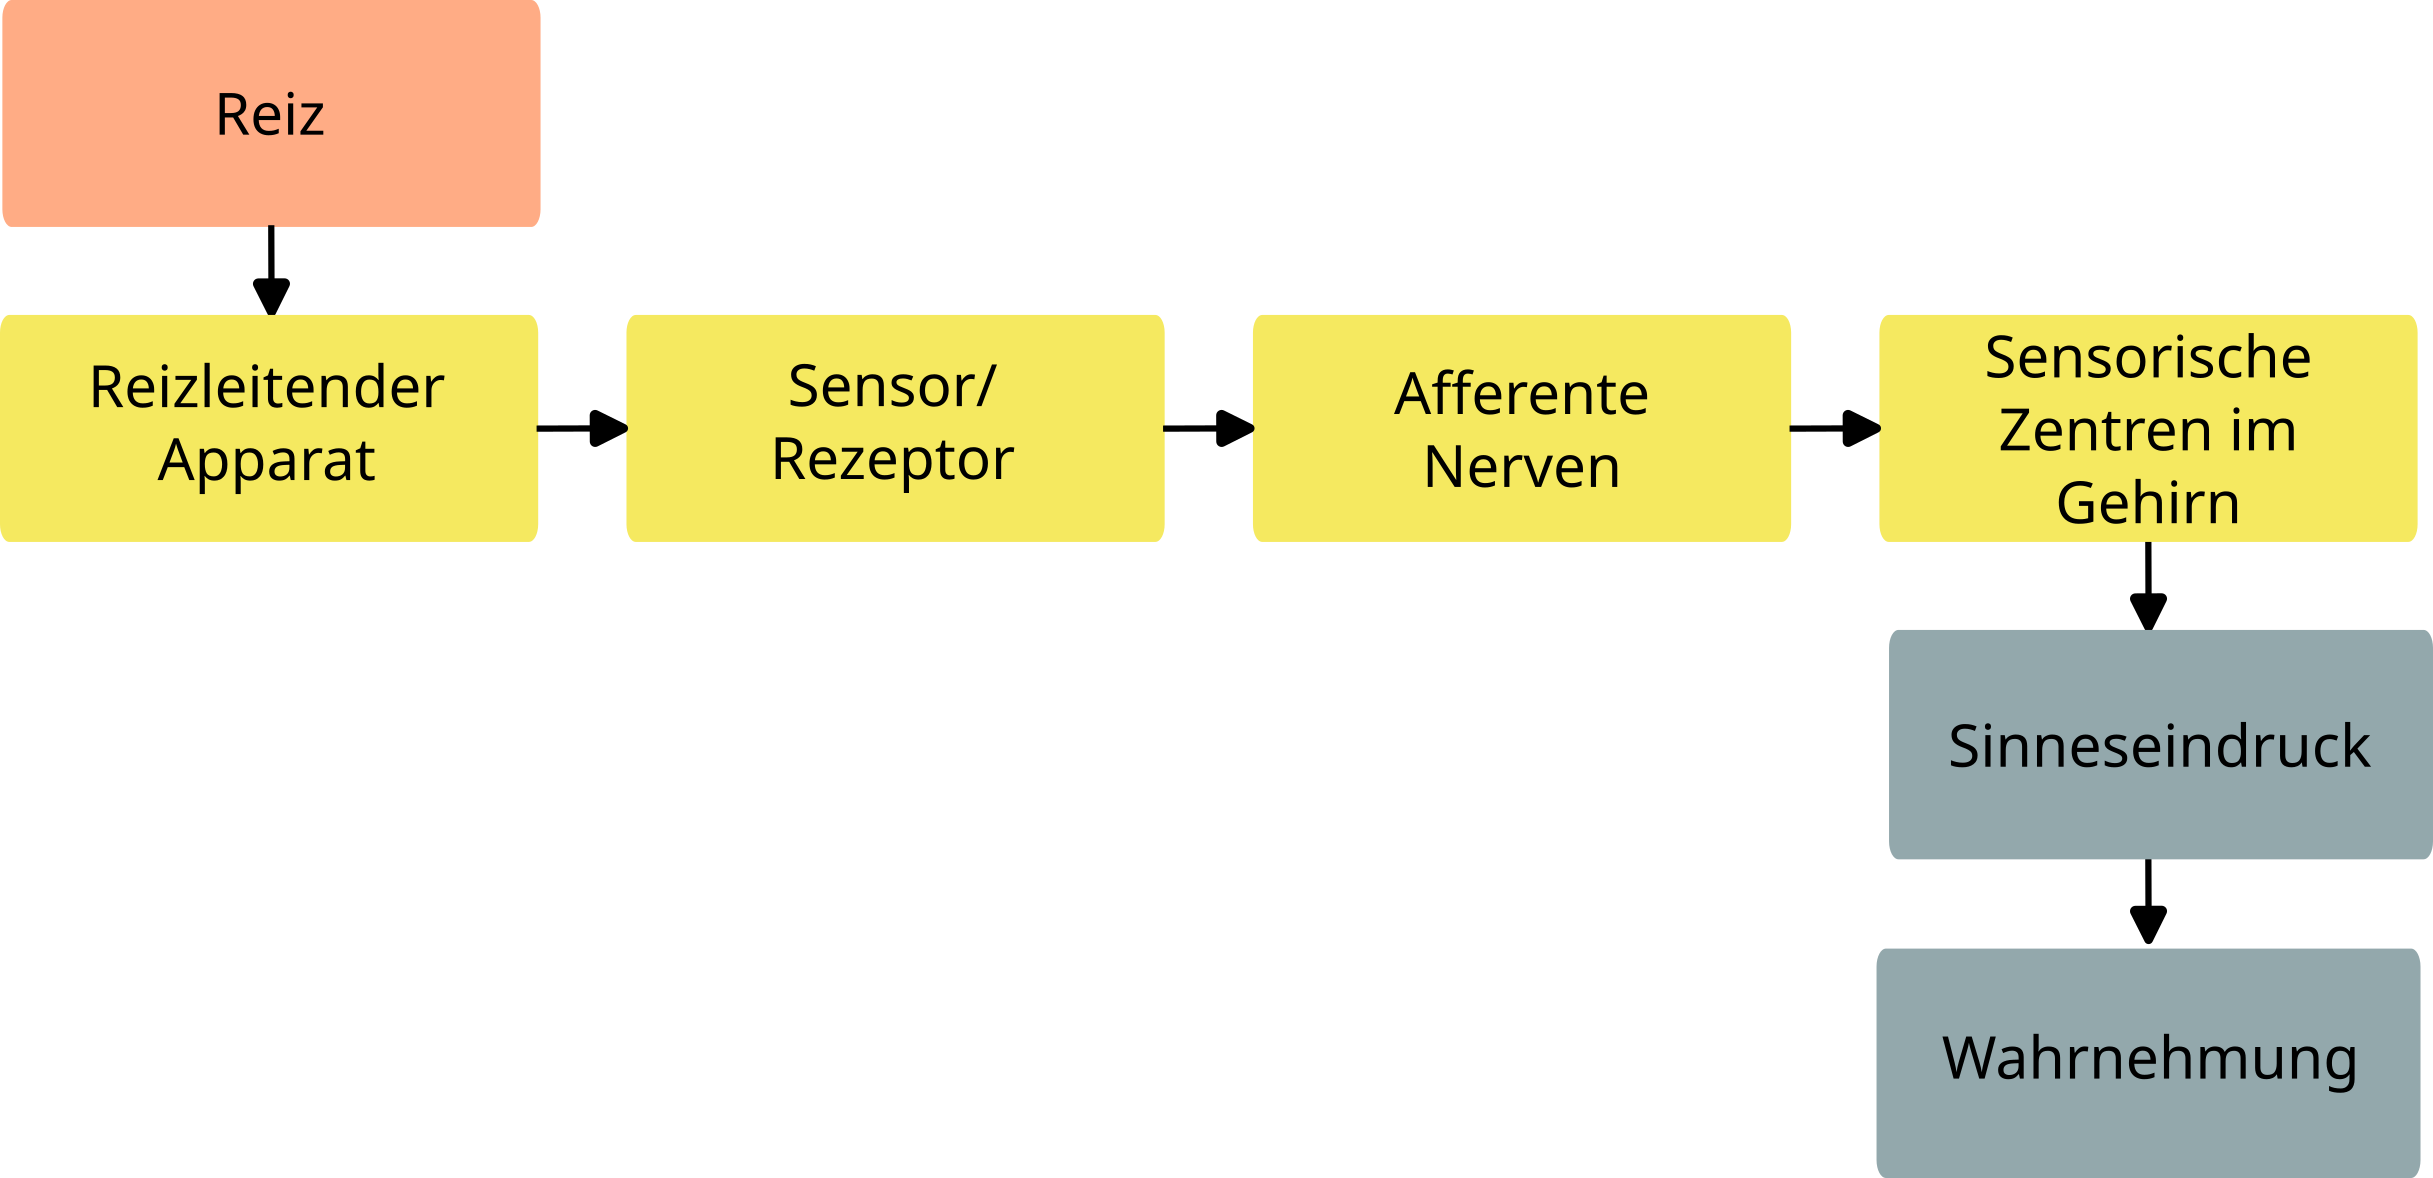
\includegraphics[width=\textwidth]{wahrnehmungsprozess_ohne_beispiel.png}
    \end{center}
    
\end{frame}

%% Reiz: 
%% Übersicht Slide
\begin{frame}{Wahrnehmungsbahn}
    
    \begin{center}
        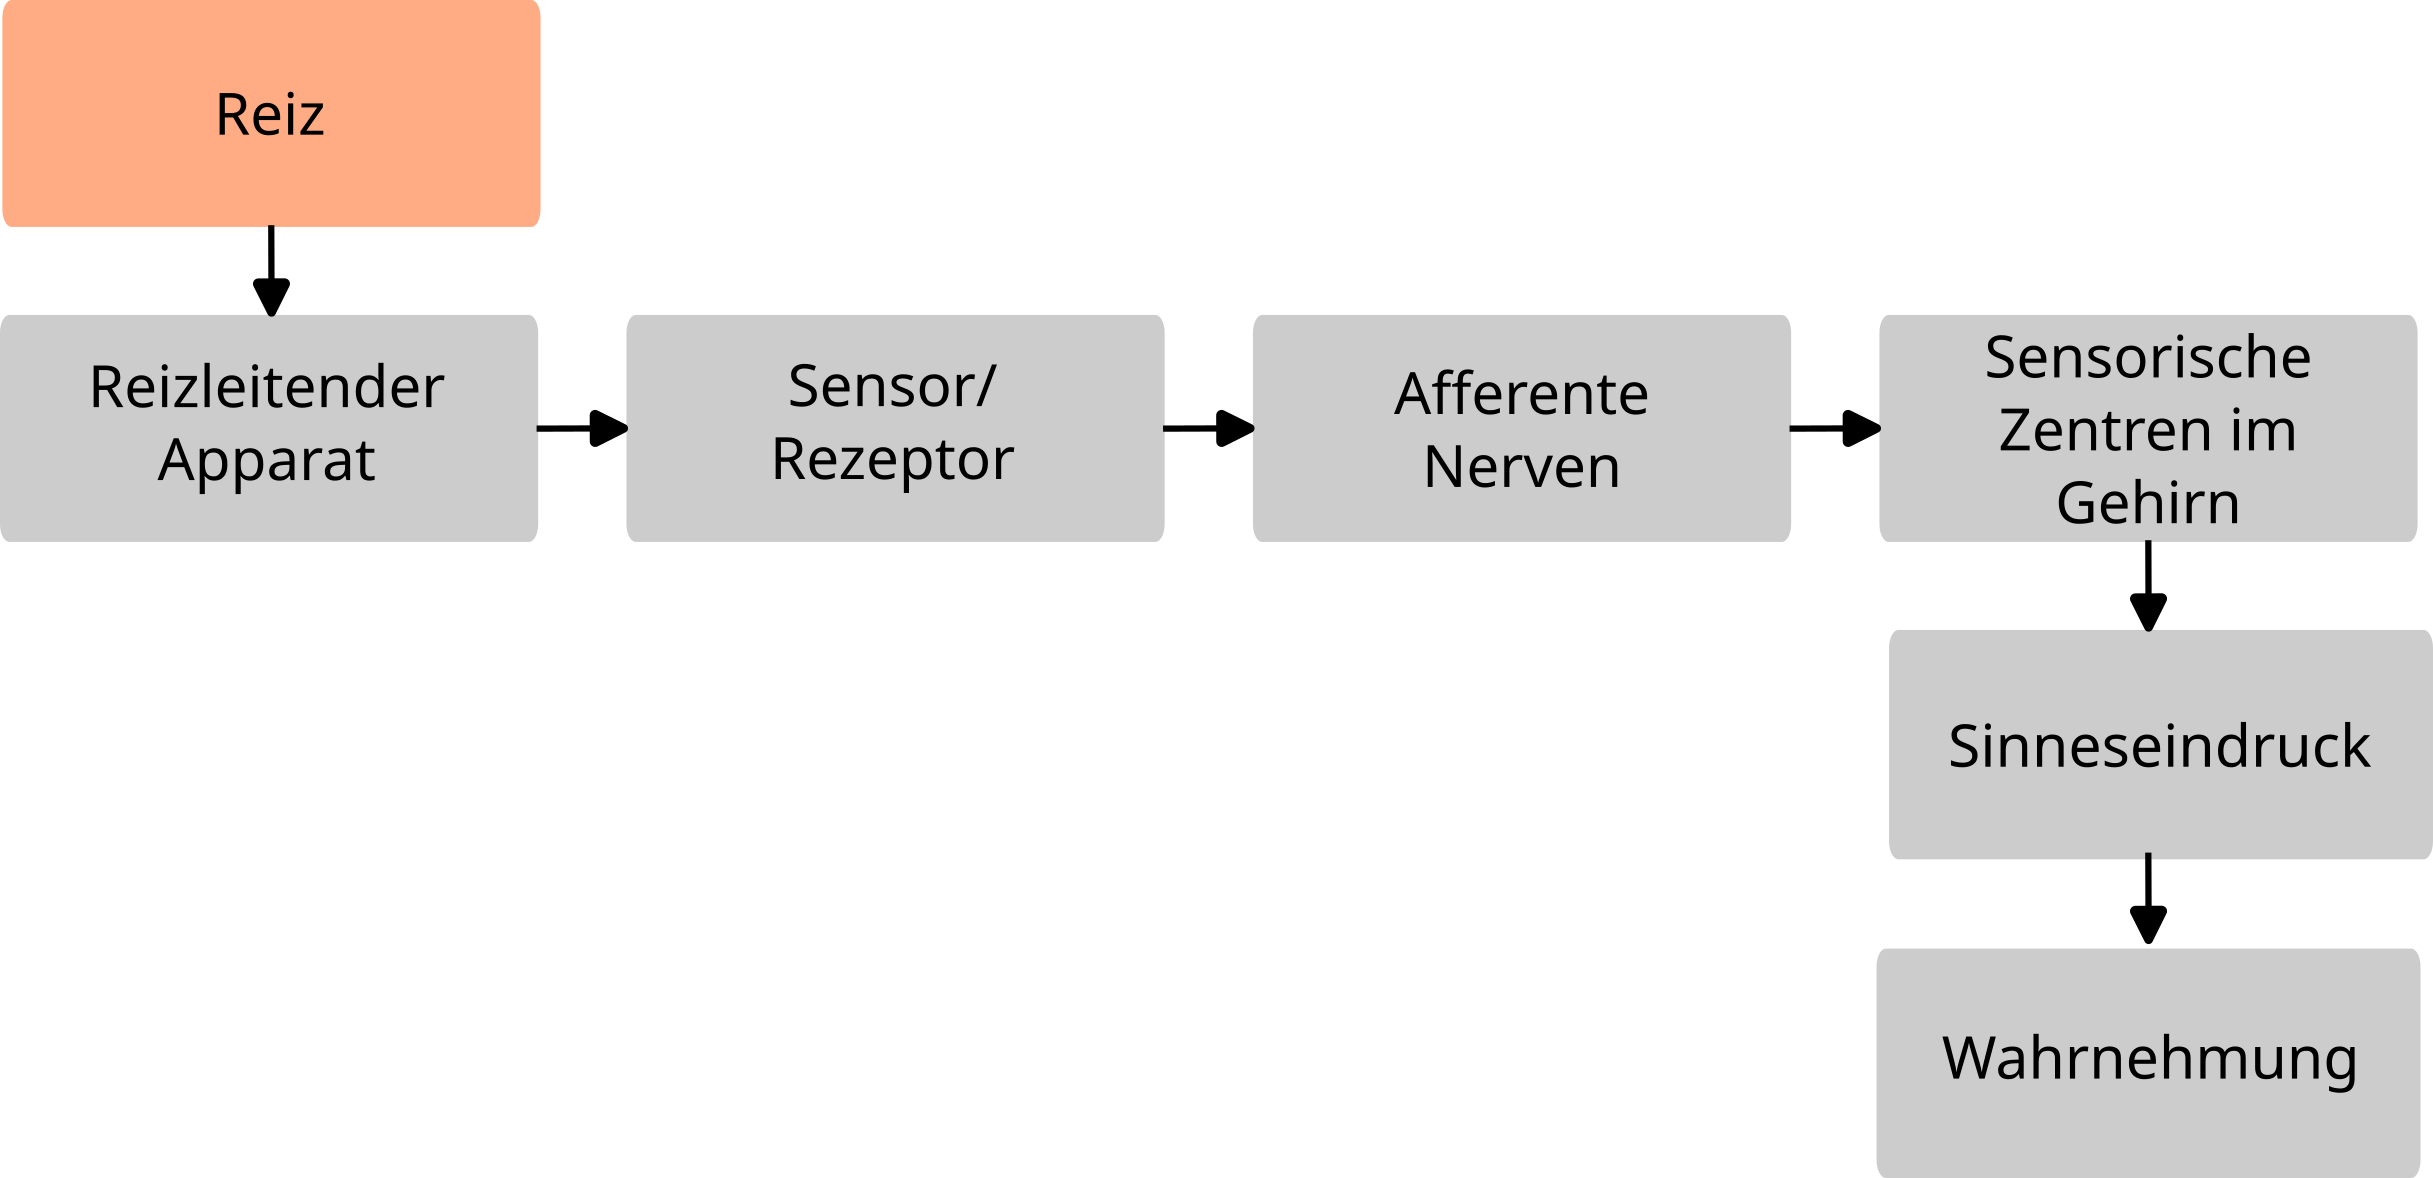
\includegraphics[width=\textwidth]{wahrnehmungsprozess_ohne_beispiel_reiz.png}
    \end{center}
    
\end{frame}




%% Schmerzreize

\begin{frame}
\frametitle{Schmerzreize}

Drei Arten von Schmerz können wahrgenommen werden:

\begin{itemize}
\item
Mechanisch (Verformung im Gewebe)
\item
Thermisch (Hitze oder Kälte)
\item
Chemisch (Körpereigene Substanzen, die z.B. bei Gewebeschäden freigesetzt werden)
\end{itemize}
\end{frame}


%% Wozu Schmerz
\begin{frame}{Wozu Schmerzen?}


\begin{columns}[c]
\begin{column}{5cm}

\begin{center}
    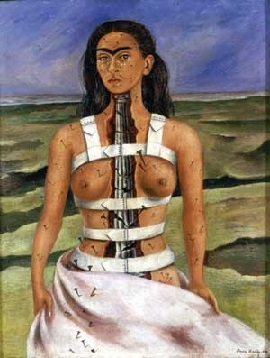
\includegraphics[width=\textwidth]{The_Broken_Column.jpg}
\end{center}

\end{column}


\pause

\begin{column}{5cm}

Warn- und Schutzfunktion \\

Einleitung von Handlungen zur Selbsterhaltung (z.B. Zurückziehen von der Schmerzquelle, Schonhaltung)

\end{column}

\end{columns}
    
\end{frame}


% Kongenitale Analgesie
\begin{frame}{Klinisches Beispiel}

\begin{block}{Kongenitale Analgesie}
\begin{itemize}
\item
Betroffene spüren keine Schmerzen
    \item 
    Extrem selten (1 in 25\,000 Lebendgeburten)
    \item
    Meist verursacht durch eine Mutation in einem spannungsaktivierten Natriumkanal (\emph{Wozu führt das?})
    \item
    Große Verletzungsgefahr, vor allem in der Kindheit 
    \item
    Nicht-Erkennen von Verletzungen und Krankheiten 
    \item
    Daher im Schnitt geringere Lebenserwartung

\end{itemize}
\end{block}


\end{frame}

%% Reizleitender Apparat und Sensor

\begin{frame}{Wahrnehmungsbahn}
    
    \begin{center}
        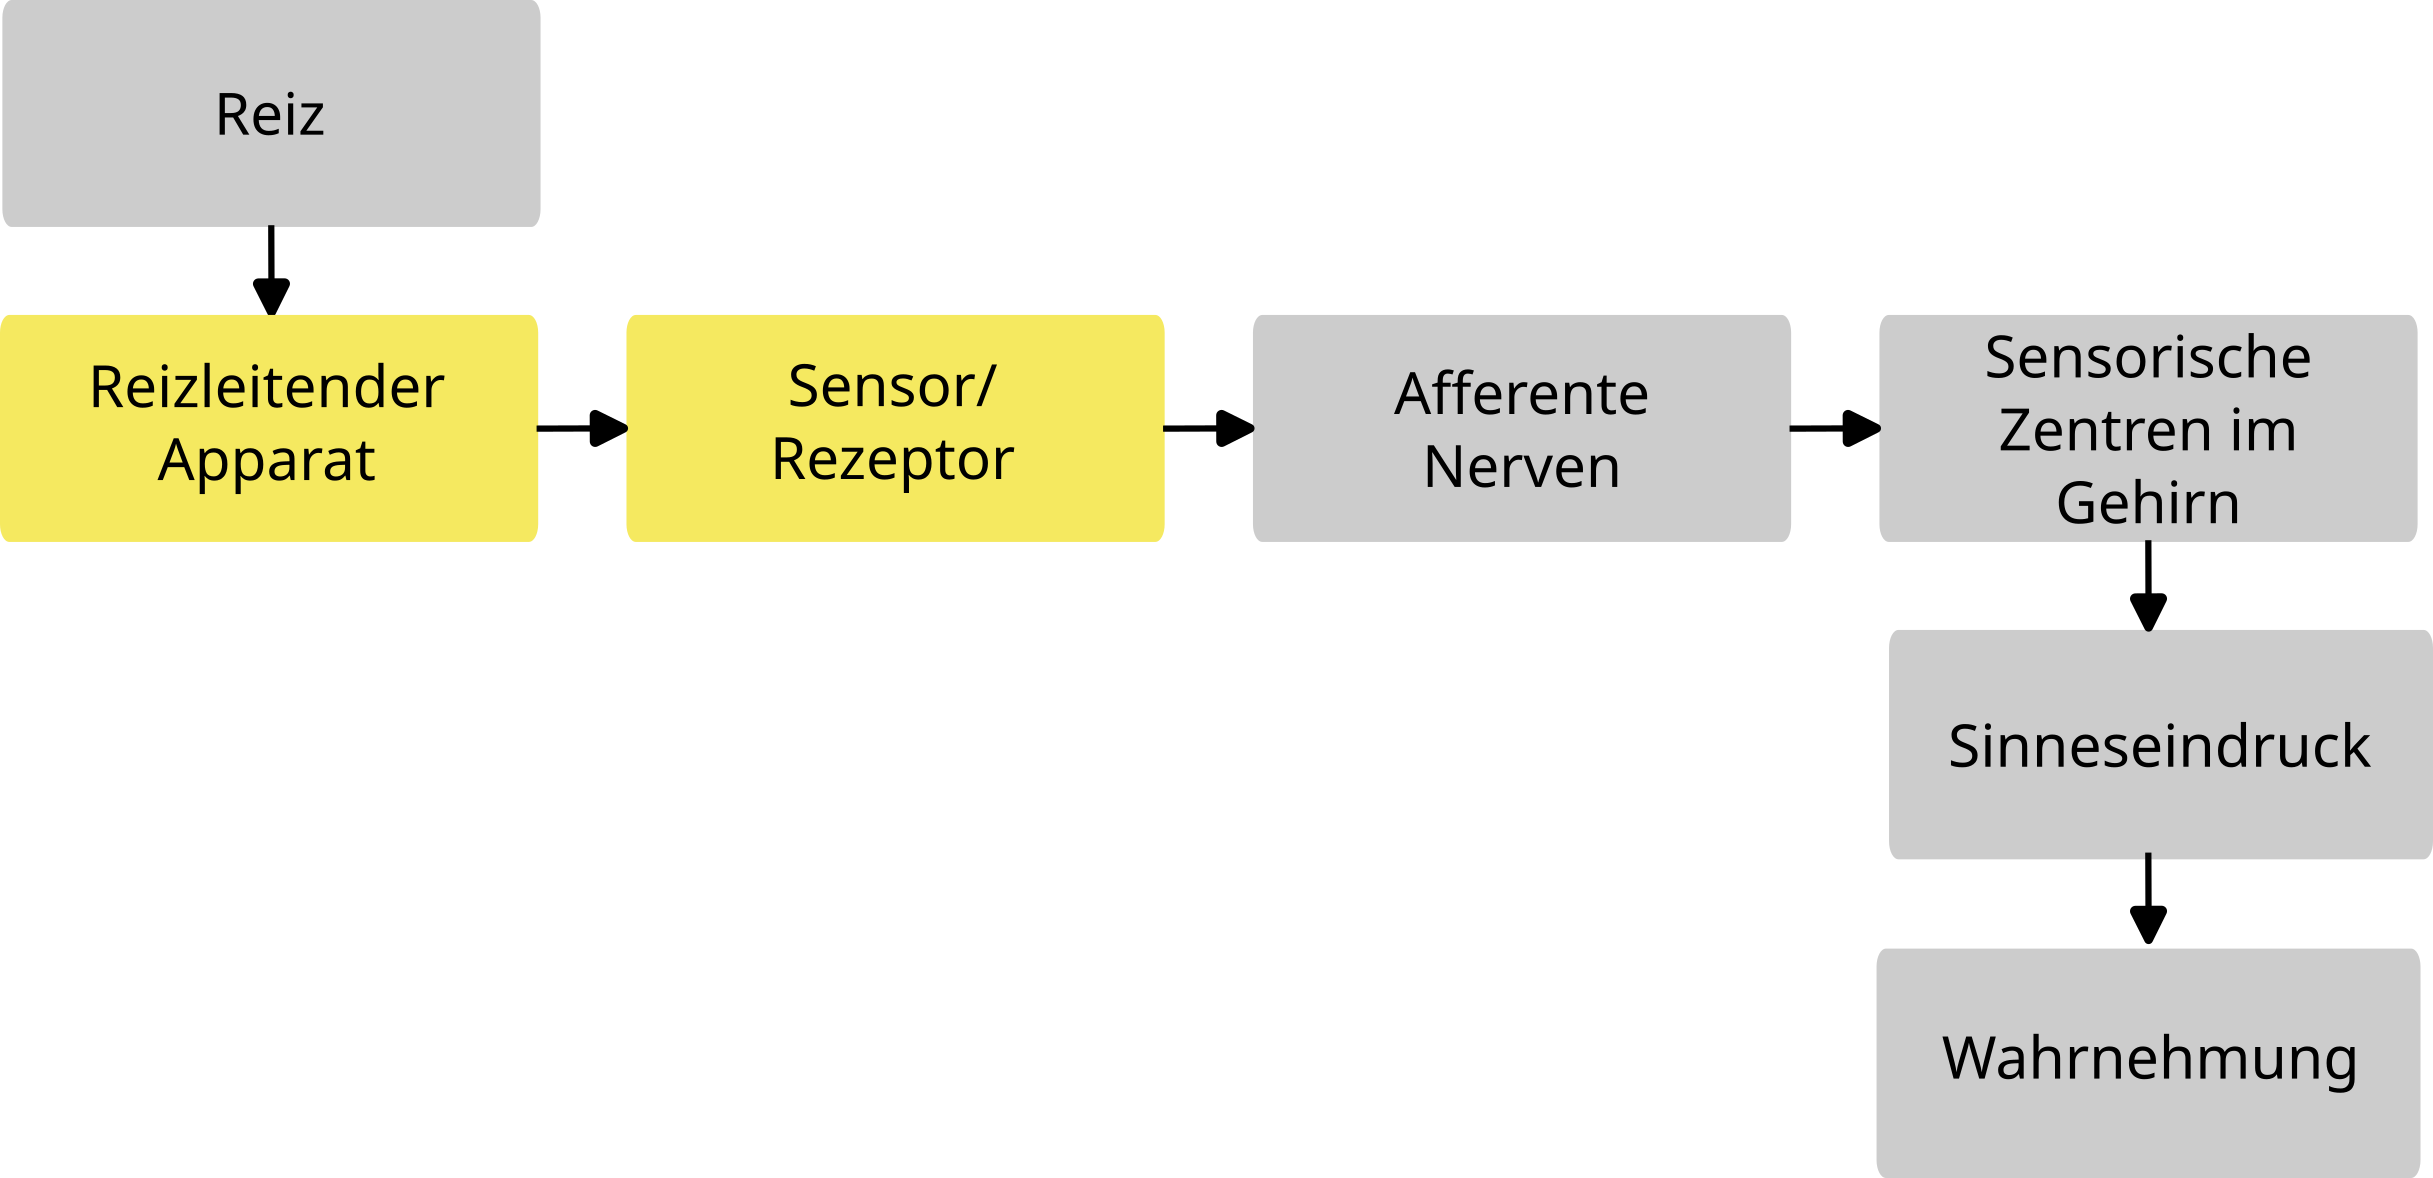
\includegraphics[width=\textwidth]{wahrnehmungsprozess_ohne_beispiel_apparat_und_sensor.png}
    
    \end{center}
    
\end{frame}


% %% Nozizeptoren: mechano, thermo, chemo
\begin{frame}
\frametitle{Nozizeptoren}


\begin{center}
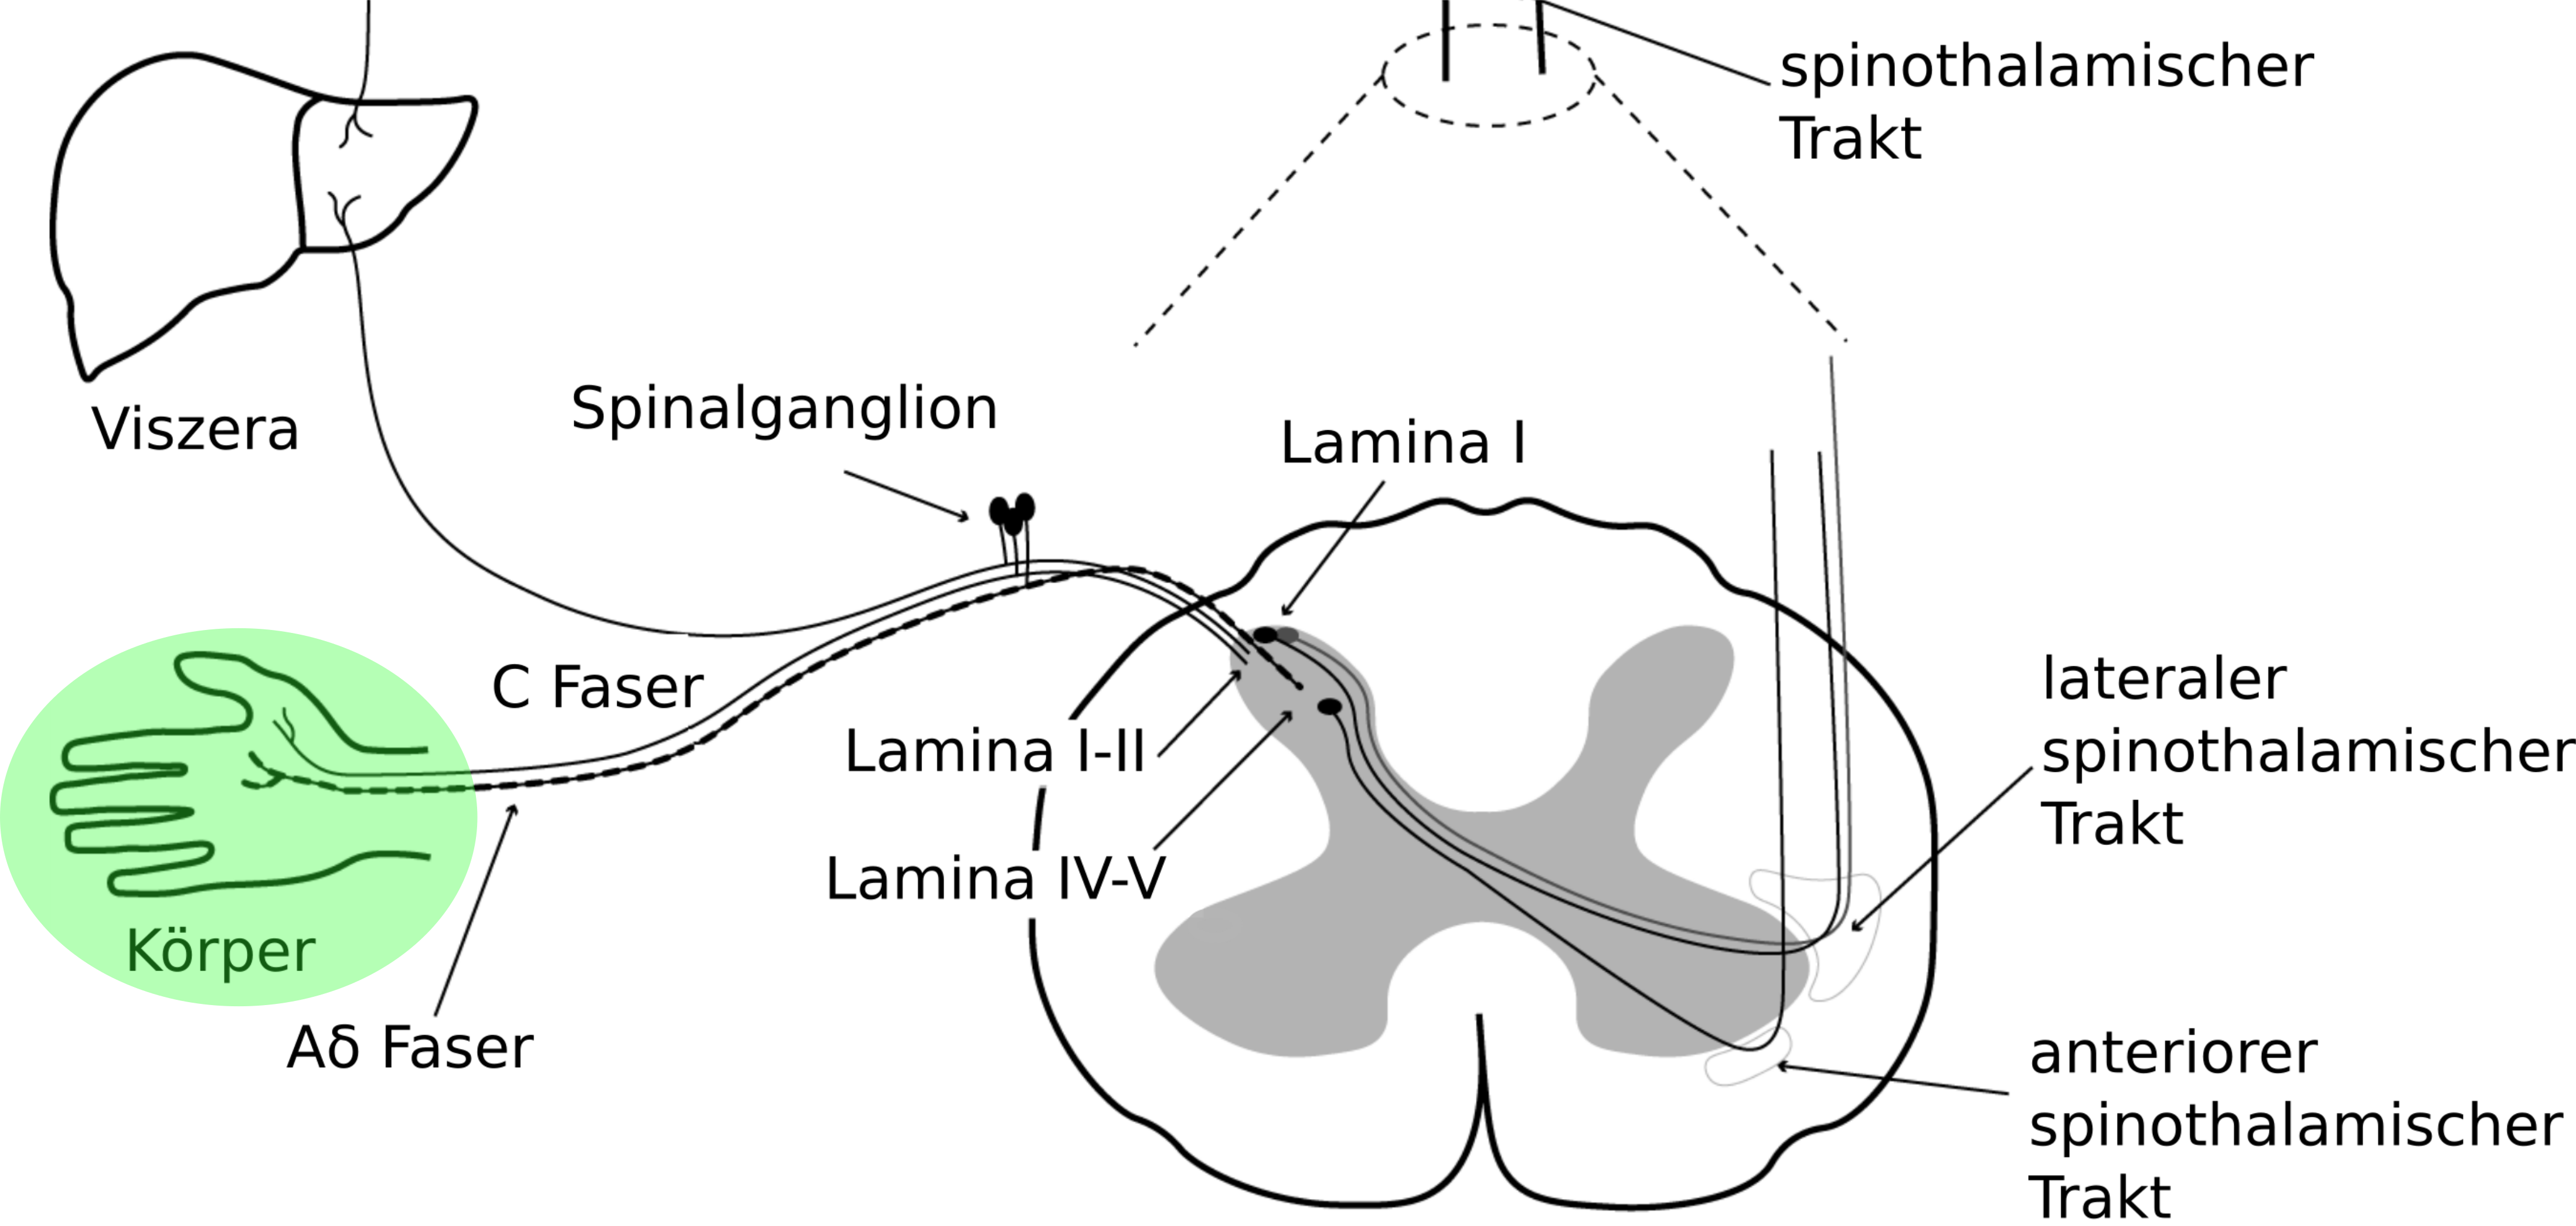
\includegraphics[width=\textwidth]{Schmerz_aufsteigend_bis_Rueckenmark_Nozizeptor.png}
\end{center}

Nozizeptoren (Schmerz-Empfänger) sind freie Nervenendigungen. Viele Nozizeptoren sind \textcolor{theme}{polymodal}, können also mehrere Arten von Schmerz empfangen. 

 
\end{frame}





\begin{frame}
\frametitle{Molekulare Mechanismen der Nozizeption}

\begin{columns}[c]

\begin{column}{7cm}
\begin{itemize}
\item
In der Membran von Nozizeptoren sitzen verschiedene Arten von Kationenkanälen 
\item
Die Ionenkanäle sind an Rezeptoren gekoppelt; Aktivierung des Rezeptors öffnet den Kanal
\end{itemize}



\end{column}

\begin{column}{5cm}
\begin{center}
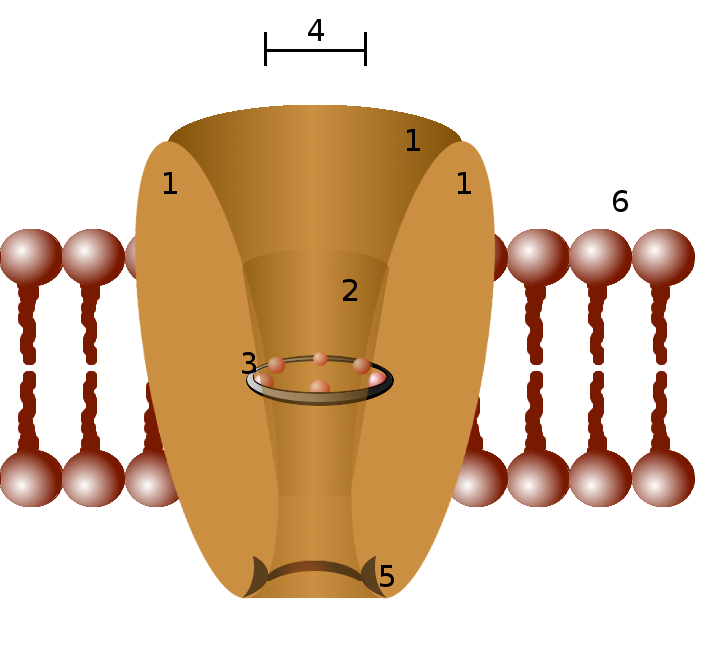
\includegraphics[width=0.7\textwidth]{Ion_channel.png}
\end{center}
\end{column}

\end{columns}

\begin{itemize}
\item
Kationen kommen in die Zelle und generieren ein Aktionspotential 
\item
Je nach Reiz unterschiedliche Rezeptoren und Kanäle und unterschiedliche Mechanismen (mechanisch, thermisch, chemisch)
\item
Manchmal wirken mehrere mögliche Reize auf denselben Rezeptor
\end{itemize}


\end{frame}


\begin{frame}
\frametitle{Was heißt "scharf" auf Englisch?}

\begin{center}
    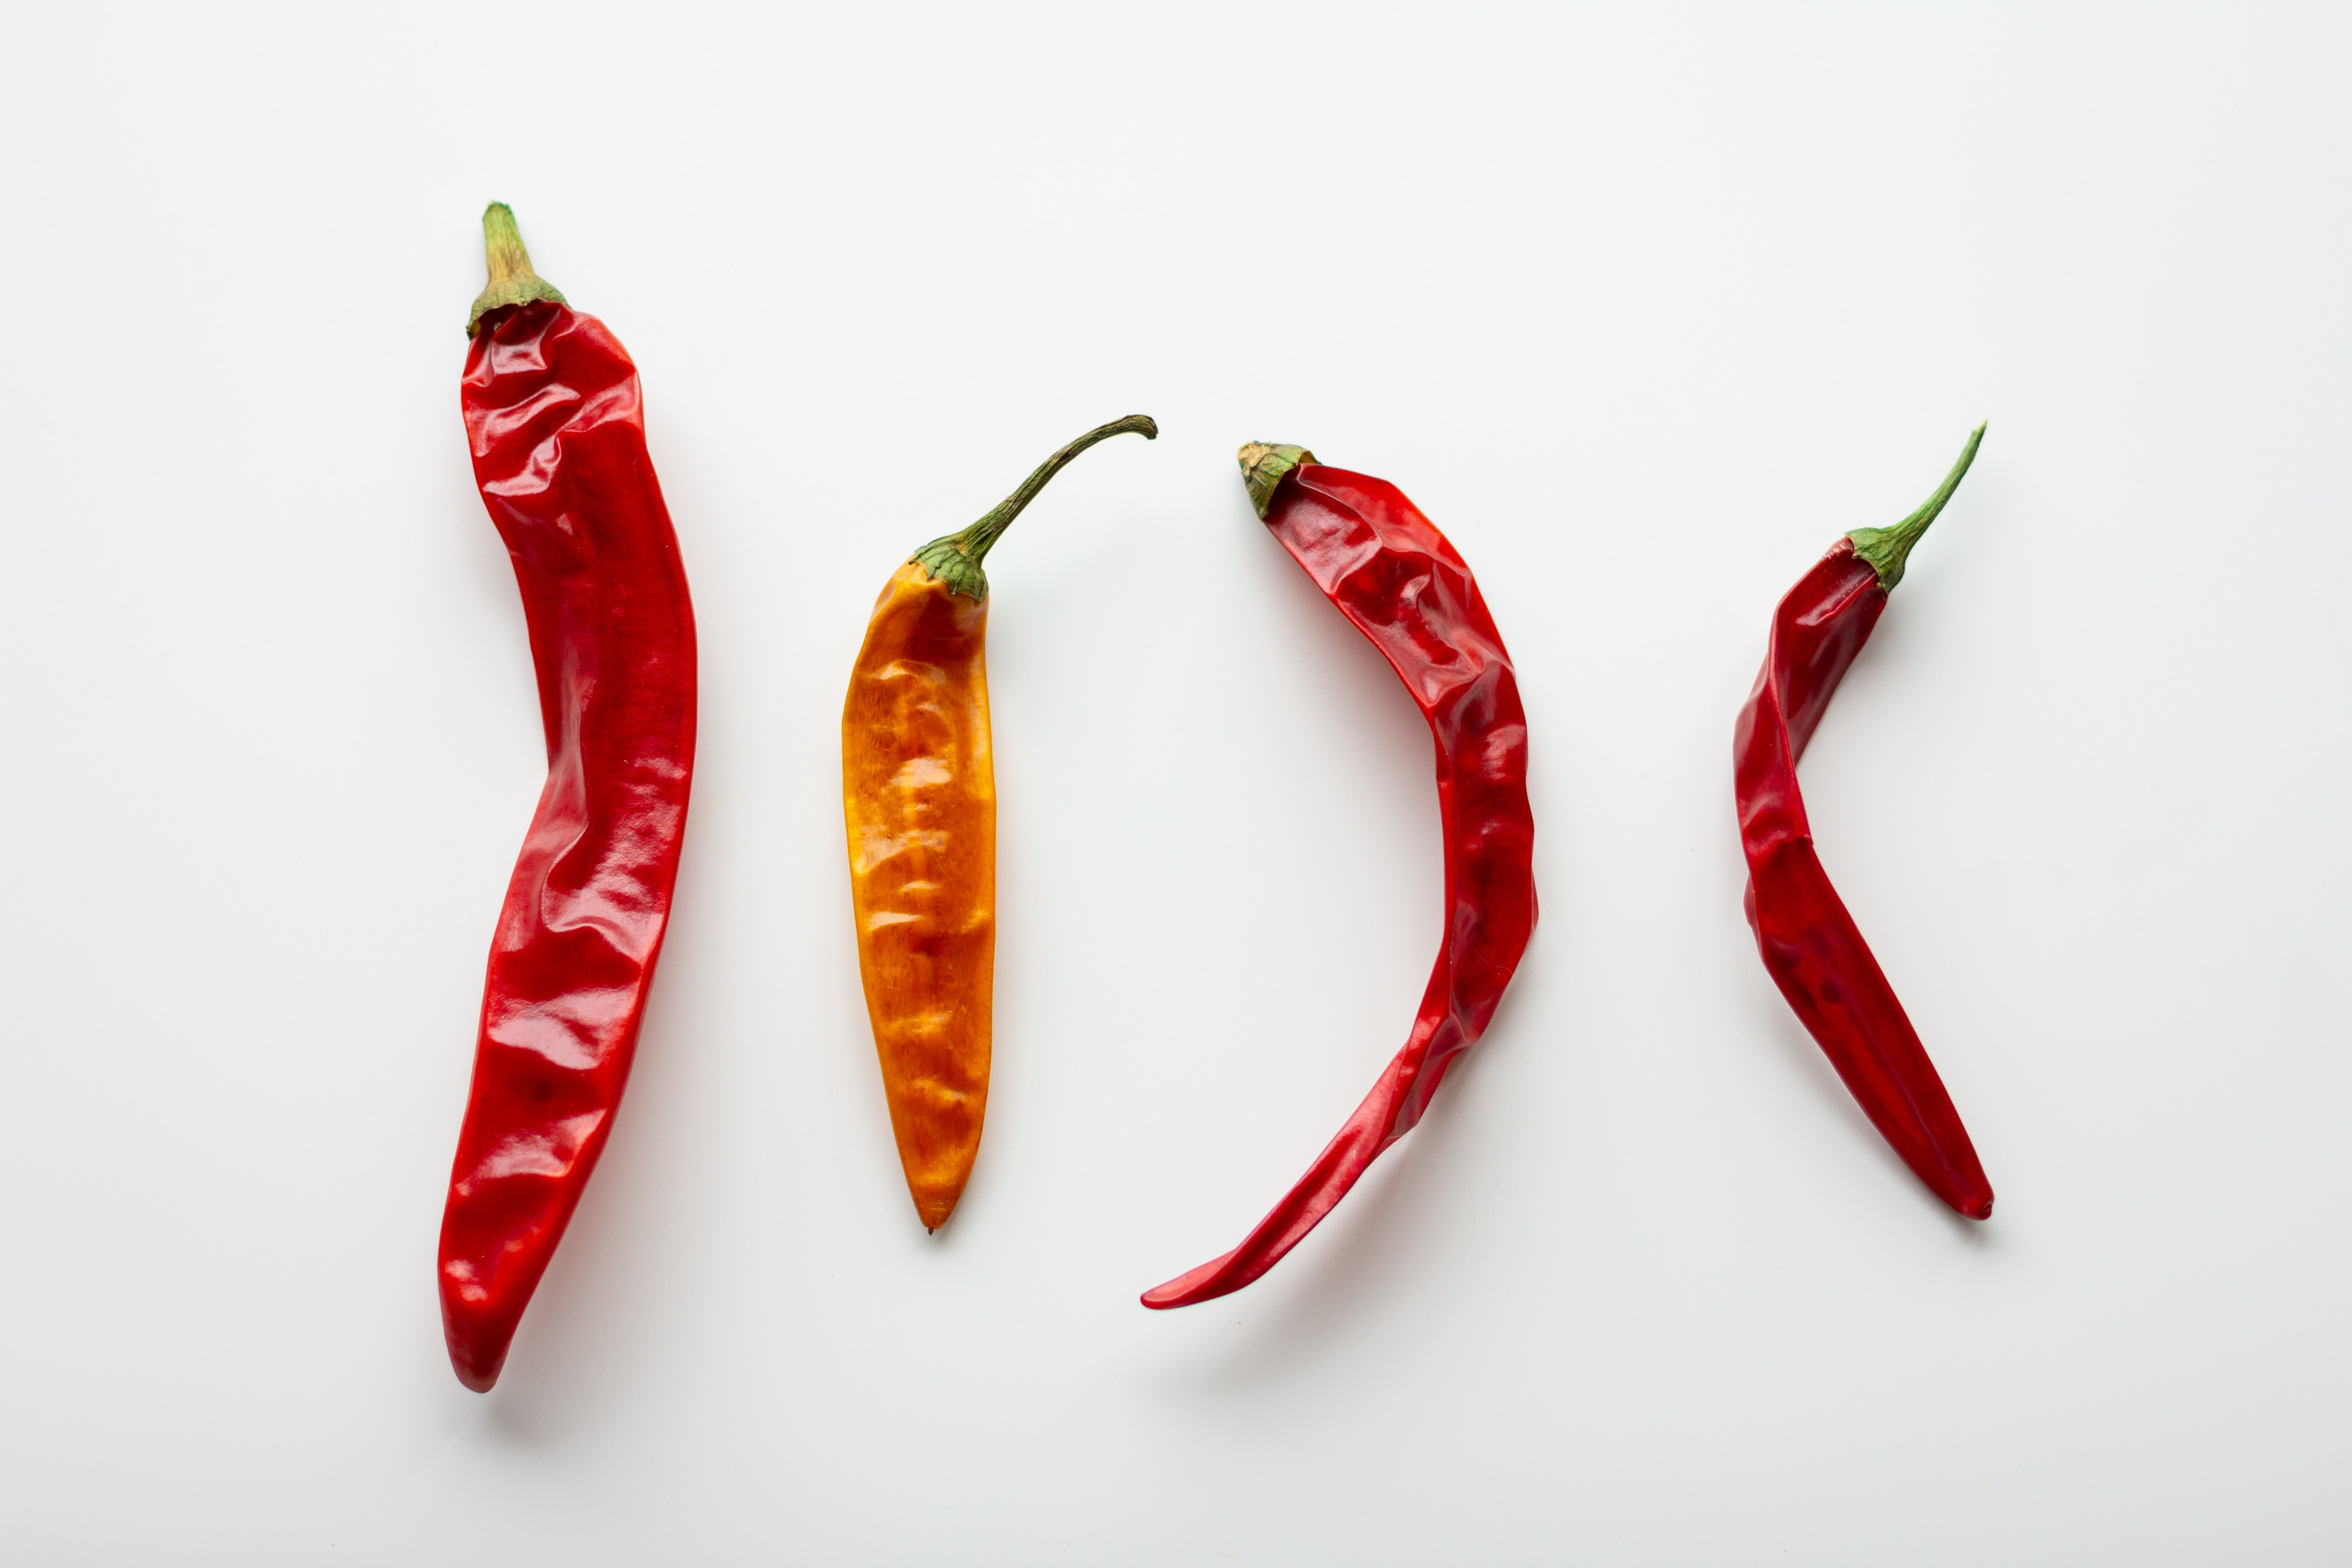
\includegraphics[width=\textwidth]{k8-innLvzxxiEg-unsplash.jpg}
\end{center}

\end{frame}

\begin{frame}
\frametitle{Beispiel: TRPV1}

\begin{center}
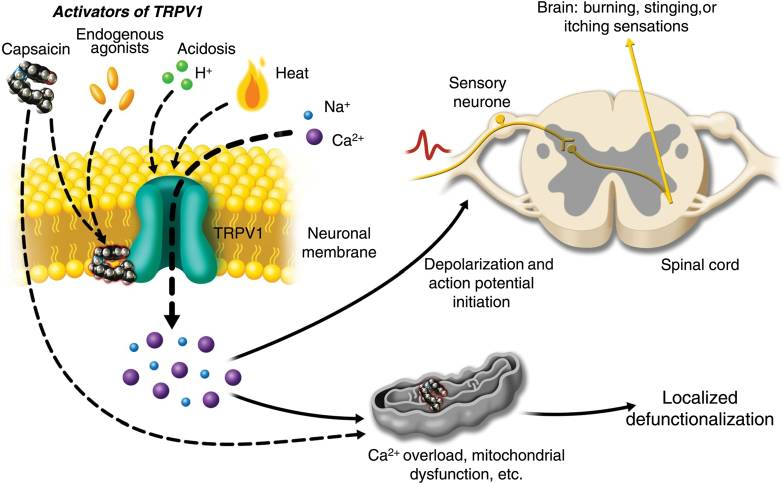
\includegraphics[width=\textwidth]{Activation_of_TRPV1_by_capsaicin.jpg}
\end{center}



\end{frame}

%% Nozizeptor-Aktivatoren: Substance P, Bradikynin


\begin{frame}
\frametitle{Manche Neuropeptide lösen chemische Nozizeption über GPCR aus}


Manche Kationenkanäle für die Schmerzwahrnehmung können durch Phosphorylierung (im innerzellulären Teil) aktiviert werden. 


\begin{center}
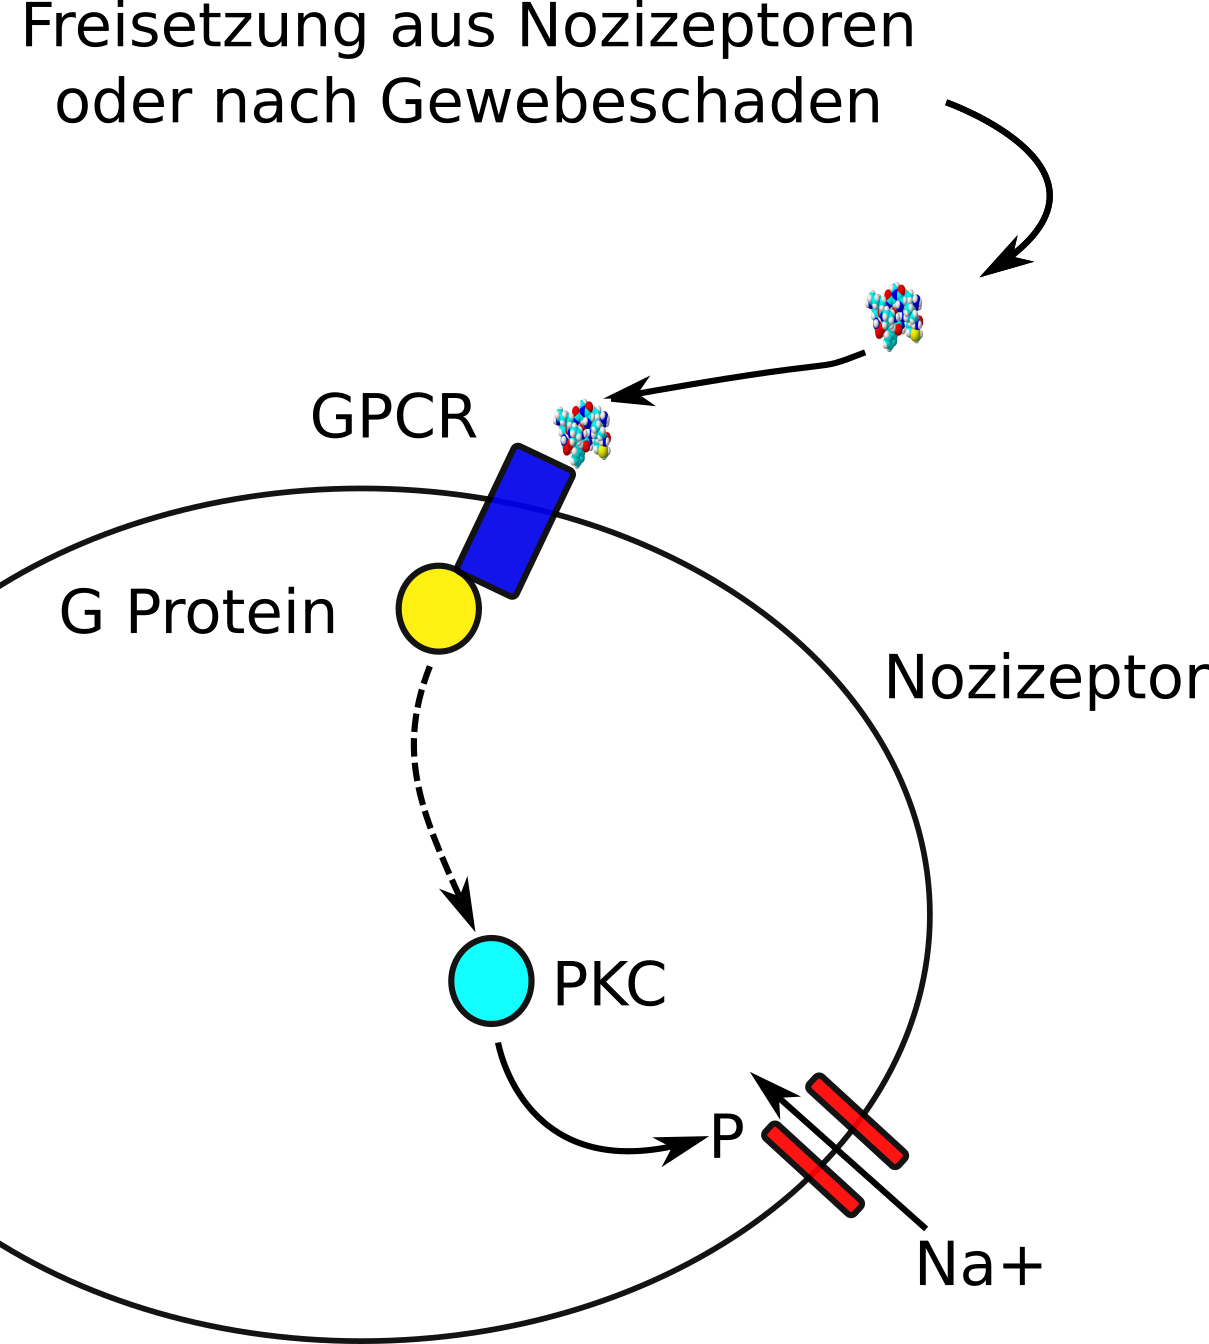
\includegraphics[width=0.4\textwidth]{nozizeptive_neuropeptide.png}
\end{center}



\end{frame}



\begin{frame}
\frametitle{Manche Neuropeptide lösen chemische Nozizeption über GPCR aus}


\begin{itemize}
\item 
Schmerz-modifizierende Substanz wird (extrazellulär) freigesetzt und trifft auf eine Nervenzelle
\item
Die Substanz bindet an einen G-Protein-gekoppelten Rezeptor (GPCR)
\item
Dies führt zur Aktivierung von G-Proteinen innerhalb der Nervenzelle und in weiterer Folge Aktivierung von Protein Kinase C (PKC)
\item
PKC phosphoryliert einen Natrium-Kanal, der dadurch geöffnet wird
\end{itemize}


\end{frame}


\begin{frame}


\frametitle{Bradykinin}

\begin{itemize}
\item
Kleines Neuropeptid (9 Aminosäuren)
\item
Wird bei Gewebeschäden freigesetzt 
\item
Verursacht eine Erweiterung der Blutgefäße und trägt damit zum Entzündungsgeschehen bei
\item
Aktiviert Nozizeptor durch Binden an einen GPCR
\end{itemize}


\end{frame}


\begin{frame}
\frametitle{Substanz P}

\begin{columns}[c]
\begin{column}{5cm}
\begin{itemize}
\item
Kleines Neuropeptid (11 Aminosäuren)
\item
Wird bei Schmerz aus Nozizeptoren freigesetzt
\item
Aktiviert den NK-1 Rezeptor (NK1R)
\item
Wie Bradykinin an Vasodilatation und Entzündungsgeschehen beteiligt 
\item 
Funktioniert nicht nur als Aktivator, sondern auch als \textcolor{theme}{Modulator} der Schmerzwahrnehmung
\end{itemize}

\end{column}

\begin{column}{5cm}
\begin{center}
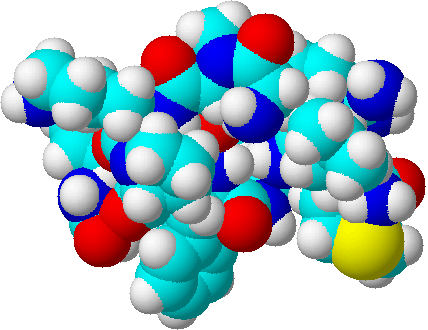
\includegraphics[width=0.7\textwidth]{Substance_P.png}
\end{center}
\end{column}
\end{columns}


\end{frame}


%% Nozizeptor-Modifikatoren (Hyperalgesie/Allodynie) - Substanz P, Prostaglandin

\begin{frame}
\frametitle{Nozizeptor-Modulatoren}

\begin{itemize}
\item
Nozizeptor-Modulatoren können einen Ionenkanal im Nozizeptor sensibilisieren.
\item
Der Ionenkanal wird dadurch nicht direkt aktiviert, aber seine Aktivierungsschwelle sinkt.
\end{itemize}

\begin{columns}[c]
\begin{column}{6.5cm}

\begin{itemize}
\item
Schmerzhafte Reize werden dadurch noch schmerzhafter (Hyperalgesie) \emph{und}

\item
Reize, die normalerweise nicht schmerzhaft sind (z.B. Berührung) können schmerzhaft werden (Allodynie)
\item
Beispiele: Substanz P, Prostaglandine
\end{itemize}
\end{column}

\begin{column}{5cm}
\begin{center}
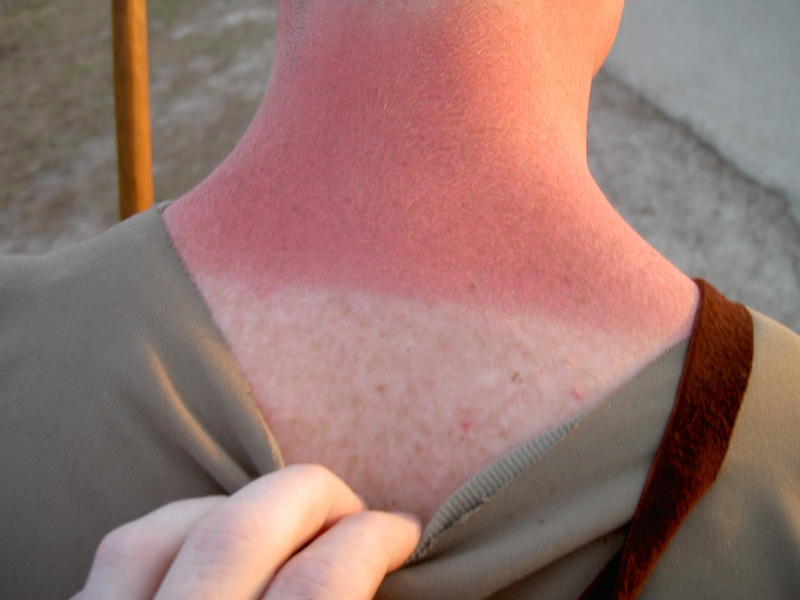
\includegraphics[width=\textwidth]{Sunburn.jpg}
\end{center}

\end{column}
\end{columns}

\end{frame}



\begin{frame}
\frametitle{Prostaglandine}

Prostaglandine entstehen z.B. bei Gewebeschaden aus dem Abbau von Phospholipiden in der Zellmembran

\pause

\begin{center}

\includegraphics[width=0.5\textwidth]{prostaglandin_synthese.png}
\end{center}



\end{frame}


%%%%%%%%%%%%%%%%%%%%%%%%%%%%%%%%%%%%%%%%
%% Afferente Nerven
%%%%%%%%%%%%%%%%%%%%%%%%%%%%%%%%%%%%%%%%

%% Übersichts-Slide

\begin{frame}{Wahrnehmungsbahn}
    
    \begin{center}
        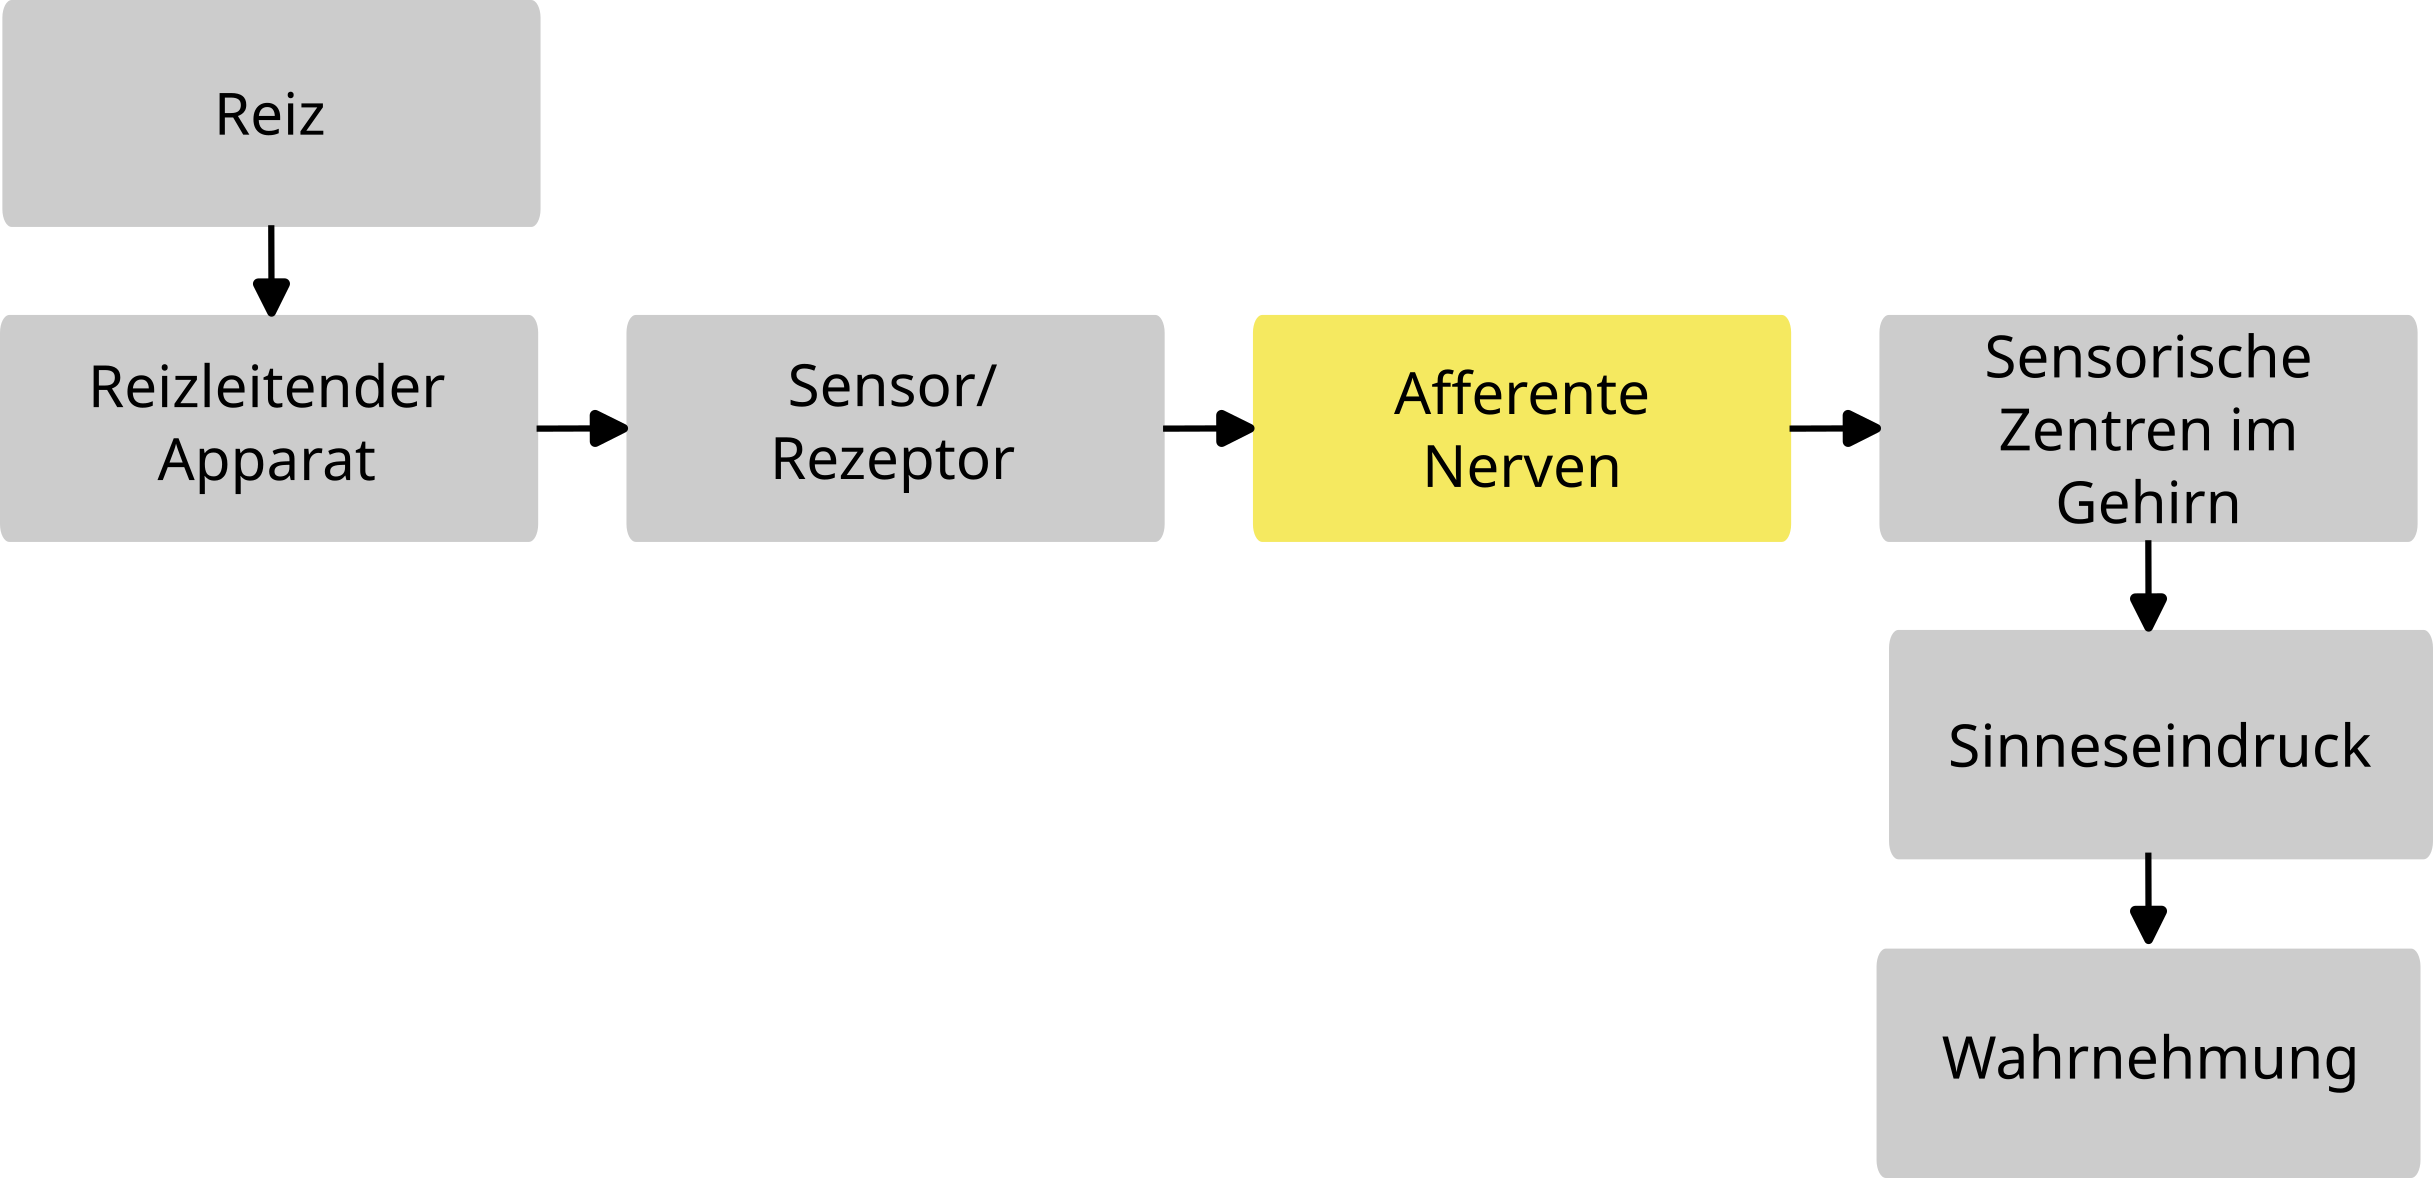
\includegraphics[width=\textwidth]{wahrnehmungsprozess_ohne_beispiel_bahnen.png}
    
    \end{center}
    
\end{frame}



%% Content aus Probevorlesung


% %% Schneller und langsamer Schmerz
\begin{frame}
\frametitle{Weiterleitung über Nervenfasern}
 
\begin{center}
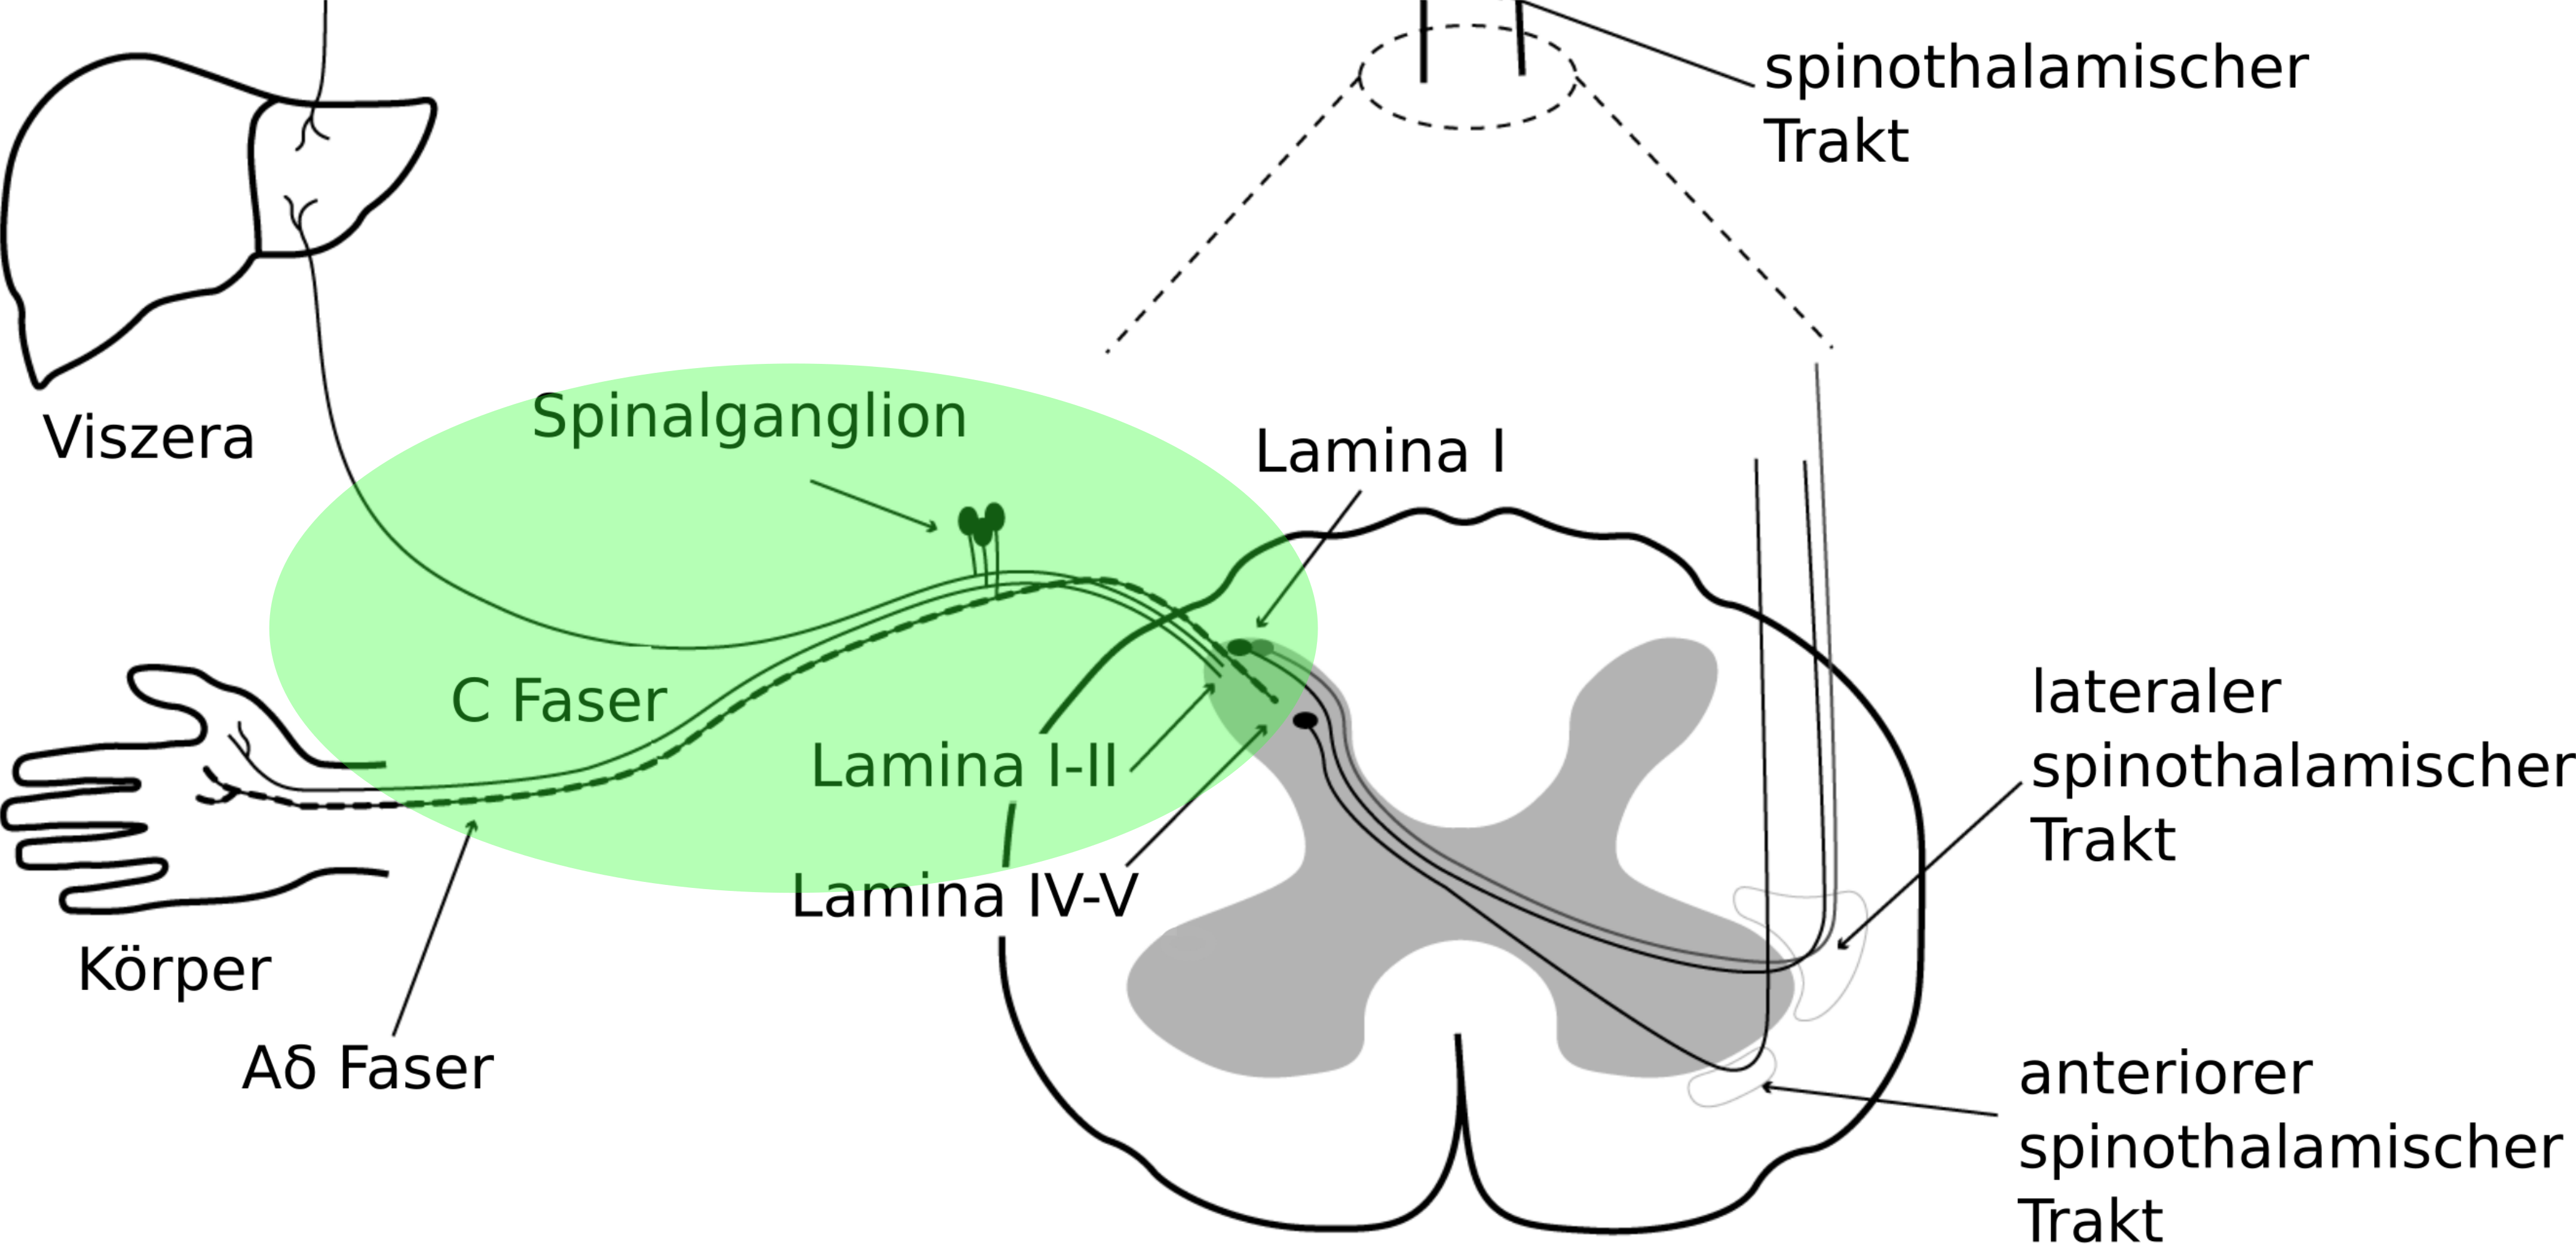
\includegraphics[width=\textwidth]{Schmerz_aufsteigend_bis_Rueckenmark_Fasern.png}
\end{center}

Der Schmerz wird ins Rückenmark weitergeleitet über A\(\delta\) (``A delta'') oder C Fasern. 

\end{frame}

\begin{frame}
\frametitle{Schneller und langsamer Schmerz}

\begin{center}

\begin{tabular}{|l|l|}
\hline
Schneller Schmerz       & Langsamer Schmerz \\
\hline
A\(\delta\) Fasern     & C Fasern \\
(myelinisiert)          & (nicht myelinisiert) \\
6-30 m/s                & 0.5-2 m/s \\
``scharf''              & ``dumpf'' \\
\hline
\end{tabular}

\end{center}


\pause


\begin{columns}[c]


\begin{column}{2.5cm}
\begin{flushright}
Joe Thomas \\
198\,cm \\
\end{flushright}
\end{column}


\begin{column}{6cm}
\begin{center}
\includegraphics[width=\textwidth]{Joe_Thomas_and_Simone_Biles.jpg}
\end{center}

\end{column}

\begin{column}{2.5cm}
Simone Biles \\
 	142\,cm  \\
\end{column}


\end{columns}



\end{frame}



\begin{frame}
\frametitle{Projizierter Schmerz}
 
\begin{center}
\includegraphics[width=0.6\textwidth]{Schmerz_aufsteigend_bis_Rueckenmark.png}
\end{center}

Innerhalb einer Faser kann nicht festgestellt werden, wo der Schmerz herkommt. Er wird daher an die Peripherie ``projiziert''.\\ 

\pause

Beispiel: Stoß auf den ``Musikantenknochen'' (Sulcus nervi ulnaris) ist als Schmerz im kleinen Finger und Ringfinger spürbar.  \\

Mögliche (aber nicht einzige) Erklärung für Phantomschmerz in amputierten Gliedmaßen. 




\end{frame}


\begin{frame}
\frametitle{Neuropathischer Schmerz}

Der Schmerz entsteht nicht wegen eines äußeren Schmerzreizes, sondern weil die Nervenfaser selber geschädigt ist, z.B. durch Virusinfektion, neurodegenerative Erkrankungen, Schlaganfall,  Diabetes mellitus, \dots  \\[1cm]

\pause

Welches Gesetz aus der Sinnesphysiologie kommt hier zum Einsatz?  \\[0.5 cm]

%% spoiler alert
\pause 

Gesetz der spezifischen Sinnesenergien. (Nicht der äußere Reiz bestimmt die Wahrnehmung, sondern die aktivierte Sinnesbahn) 
%% end spoiler alert


\end{frame}


%% Spinal cord - dorsales Horn, vorderseitenstrang Pathway, chirurgische Eingriffe
\begin{frame}
\frametitle{Umschaltung im Rückenmark}

\begin{center}
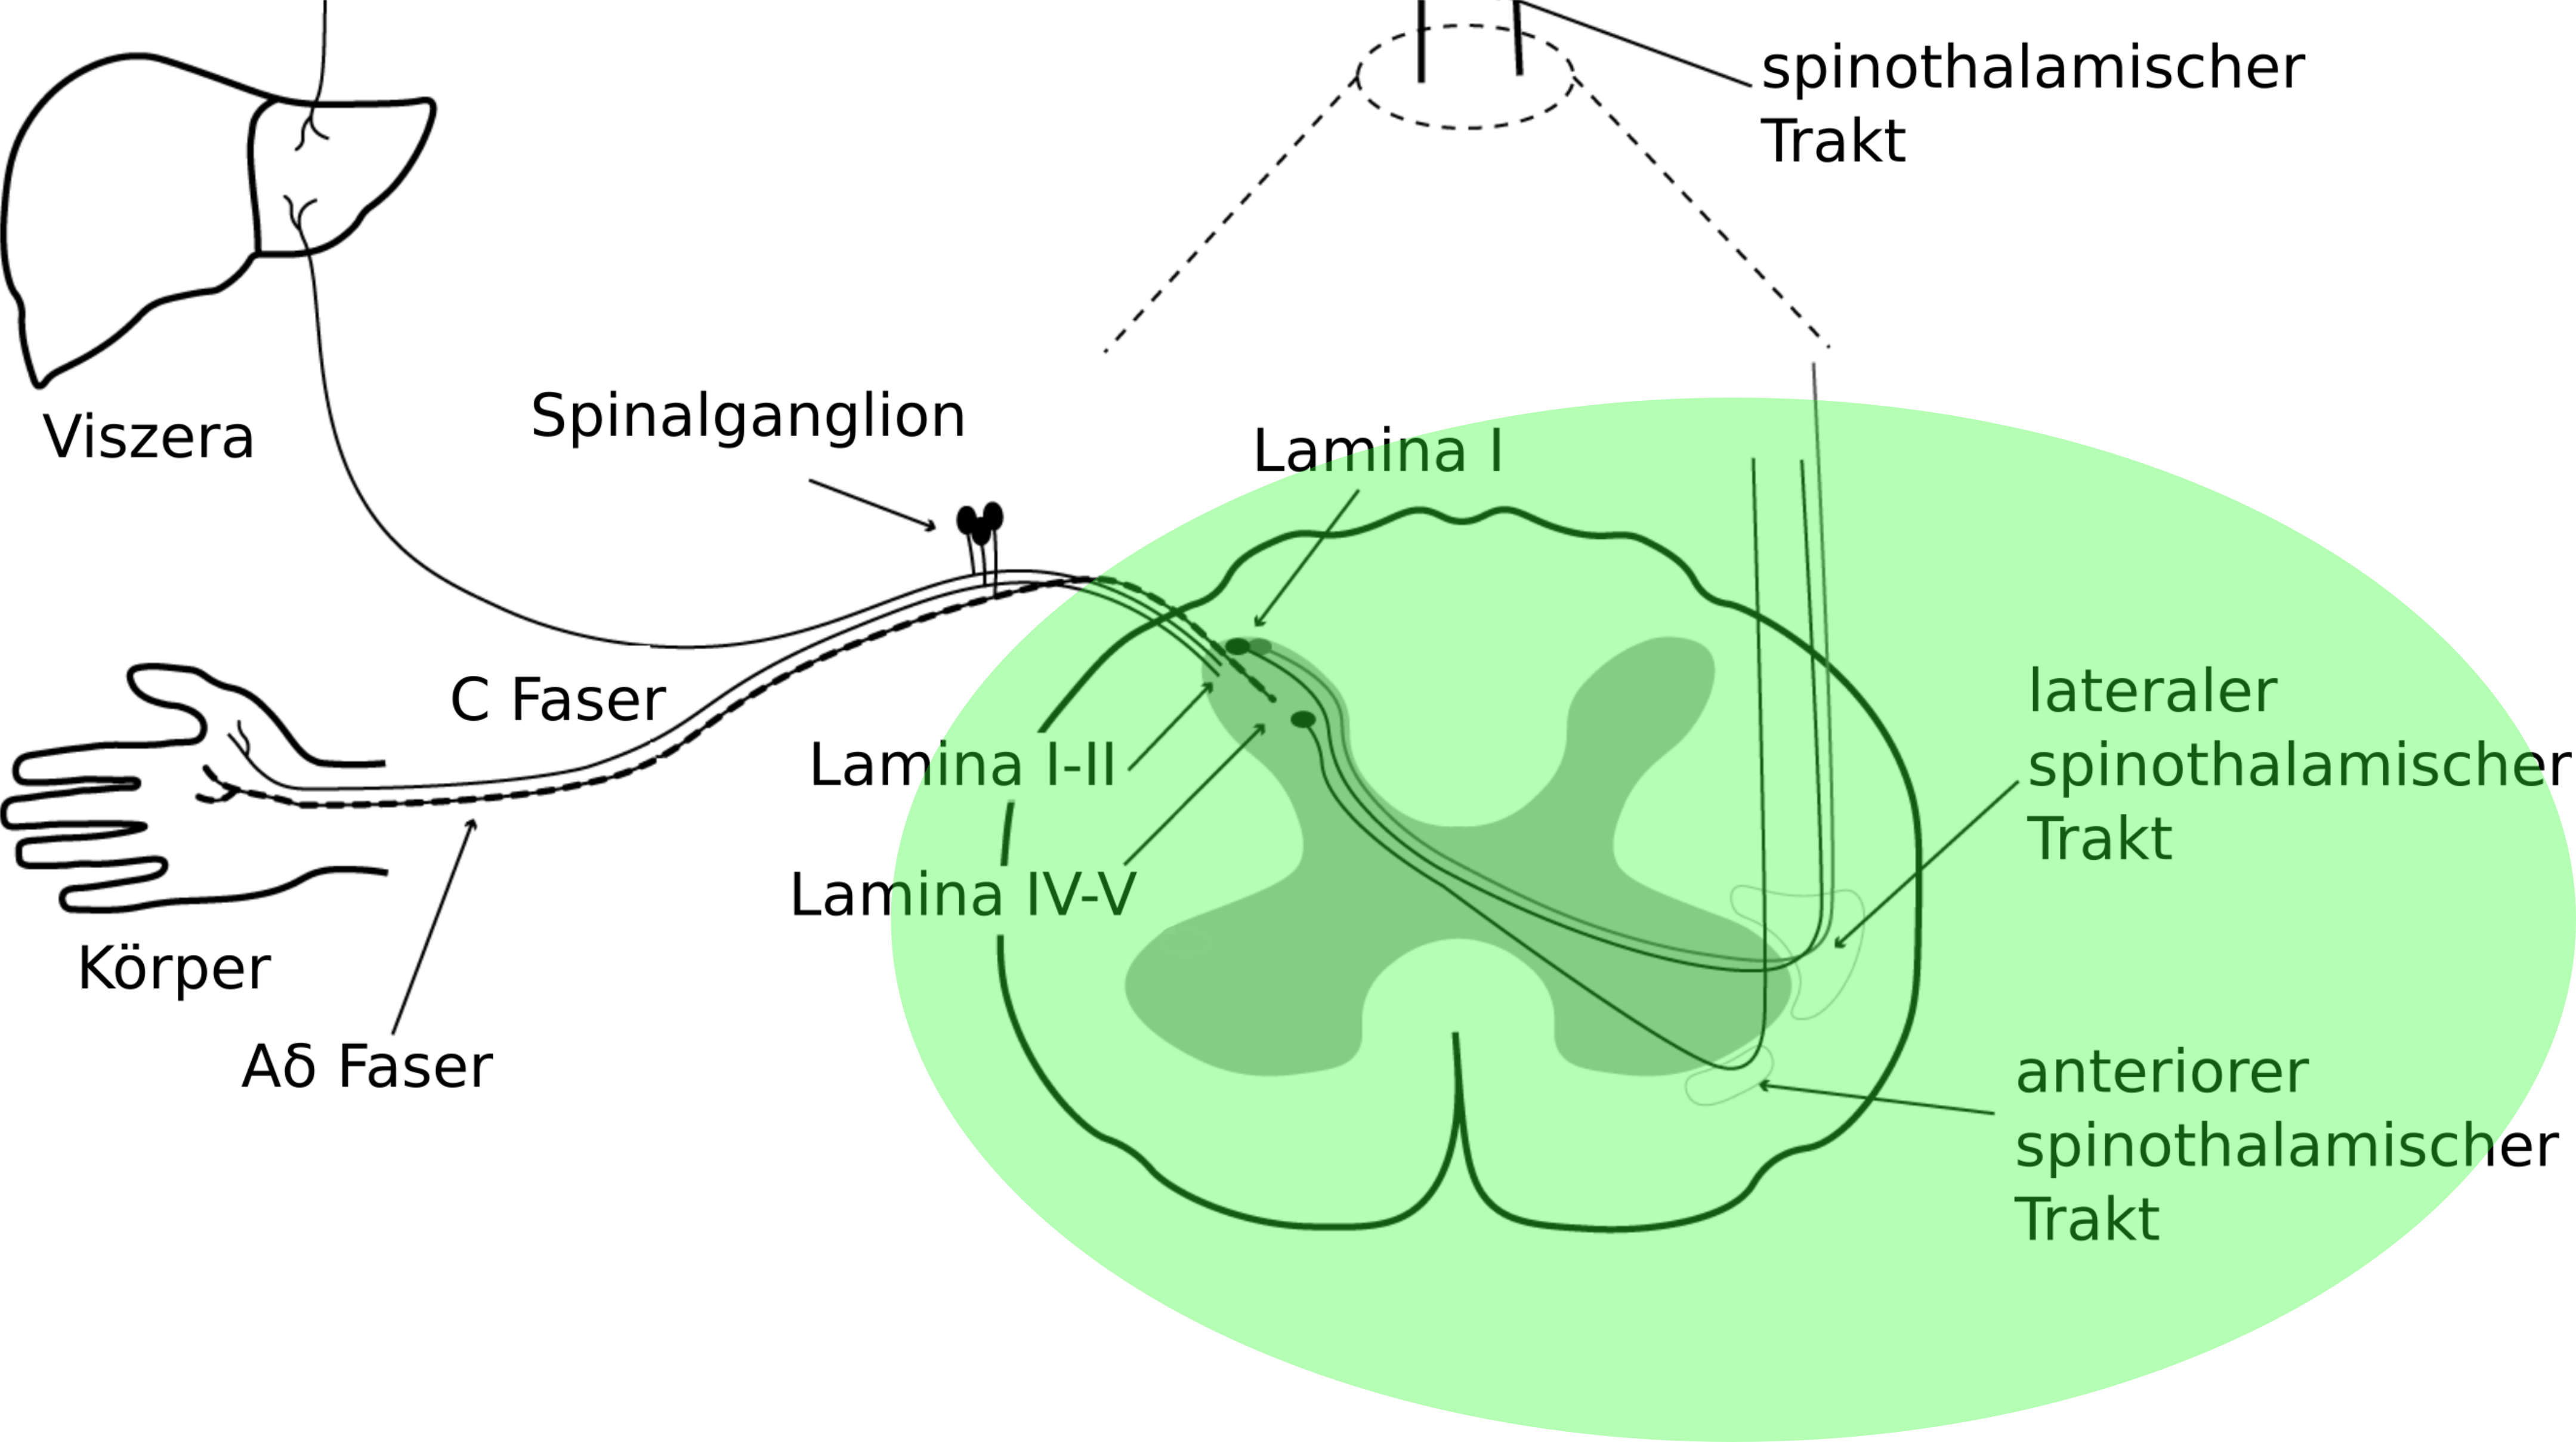
\includegraphics[width=0.8\textwidth]{Schmerz_aufsteigend_bis_Rueckenmark_Rueckenmark.png}
\end{center}

\pause

Schmerzfasern kommen durch das Rückenhorn ins Rückenmark. Hier wird das Schmerzsignal umgeschaltet (diagonal nach vorne). Es geht von dort in den Thalamus durch den tractus spinothalamicus (Vorderseitenstrang). 

\end{frame}


\begin{frame}

\frametitle{Viszeraler Schmerz}

 \begin{center}
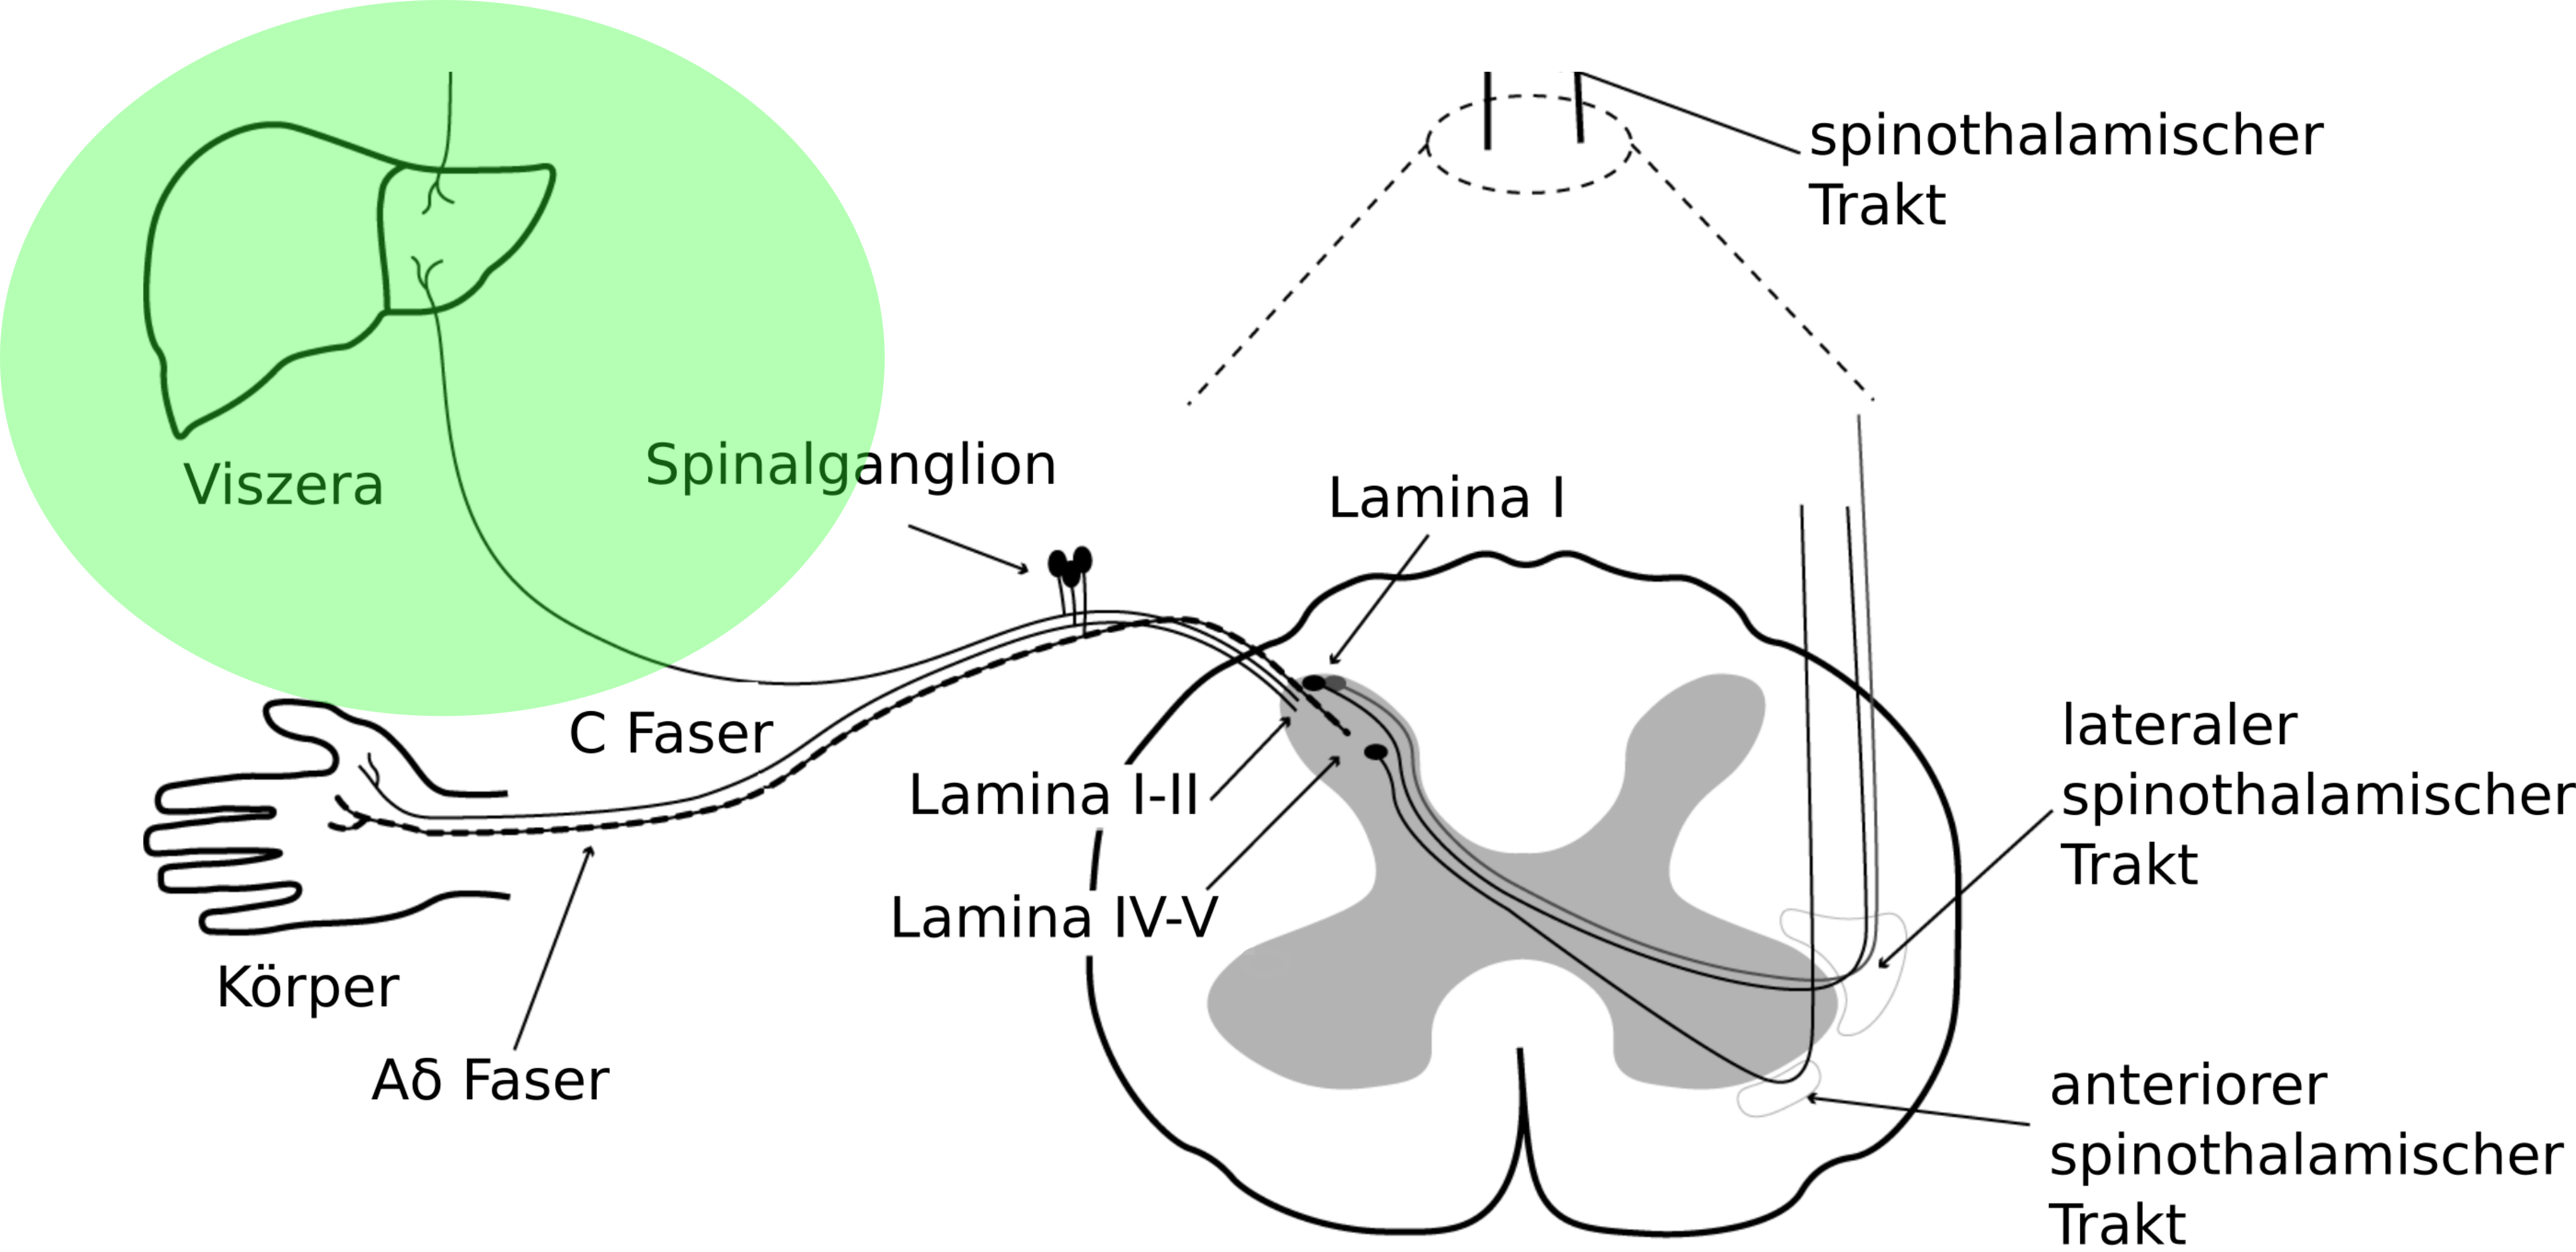
\includegraphics[width=\textwidth]{Schmerz_aufsteigend_bis_Rueckenmark_Viszera.png}
\end{center}


\end{frame}

%% Viszeraler Schmerz - Head-Zonen  
\begin{frame}
\frametitle{Viszeraler Schmerz}

\begin{columns}[c]


\begin{column}{5cm}
Schmerzen in Eingeweiden (Viszera) entstehen oft durch
 
\begin{itemize}
\item
Verformung
\item
Ischämie (Unterdurchblutung)
\item
Entzündung
\end{itemize}
\end{column}

\begin{column}{5cm}
\begin{center}
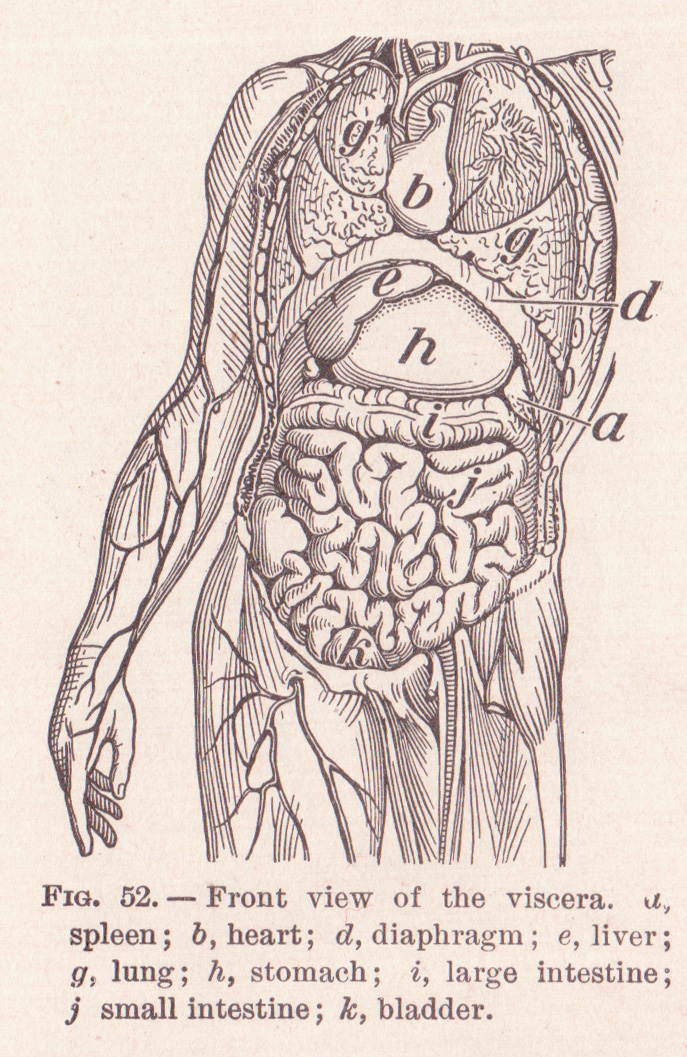
\includegraphics[width=\textwidth]{viscera.jpg}
\end{center}

\end{column}

\end{columns}


\end{frame}

\begin{frame}
\frametitle{Übertragener Schmerz}

Viszeraler Schmerz wird oft als Oberflächenschmerz in anderen Regionen des Körpers wahrgenommen (``übertragener Schmerz'') \\
Die Entsprechungen sind als ``Head-Zonen'' (auch ``Head'sche Zonen'') kartiert.


\begin{center}
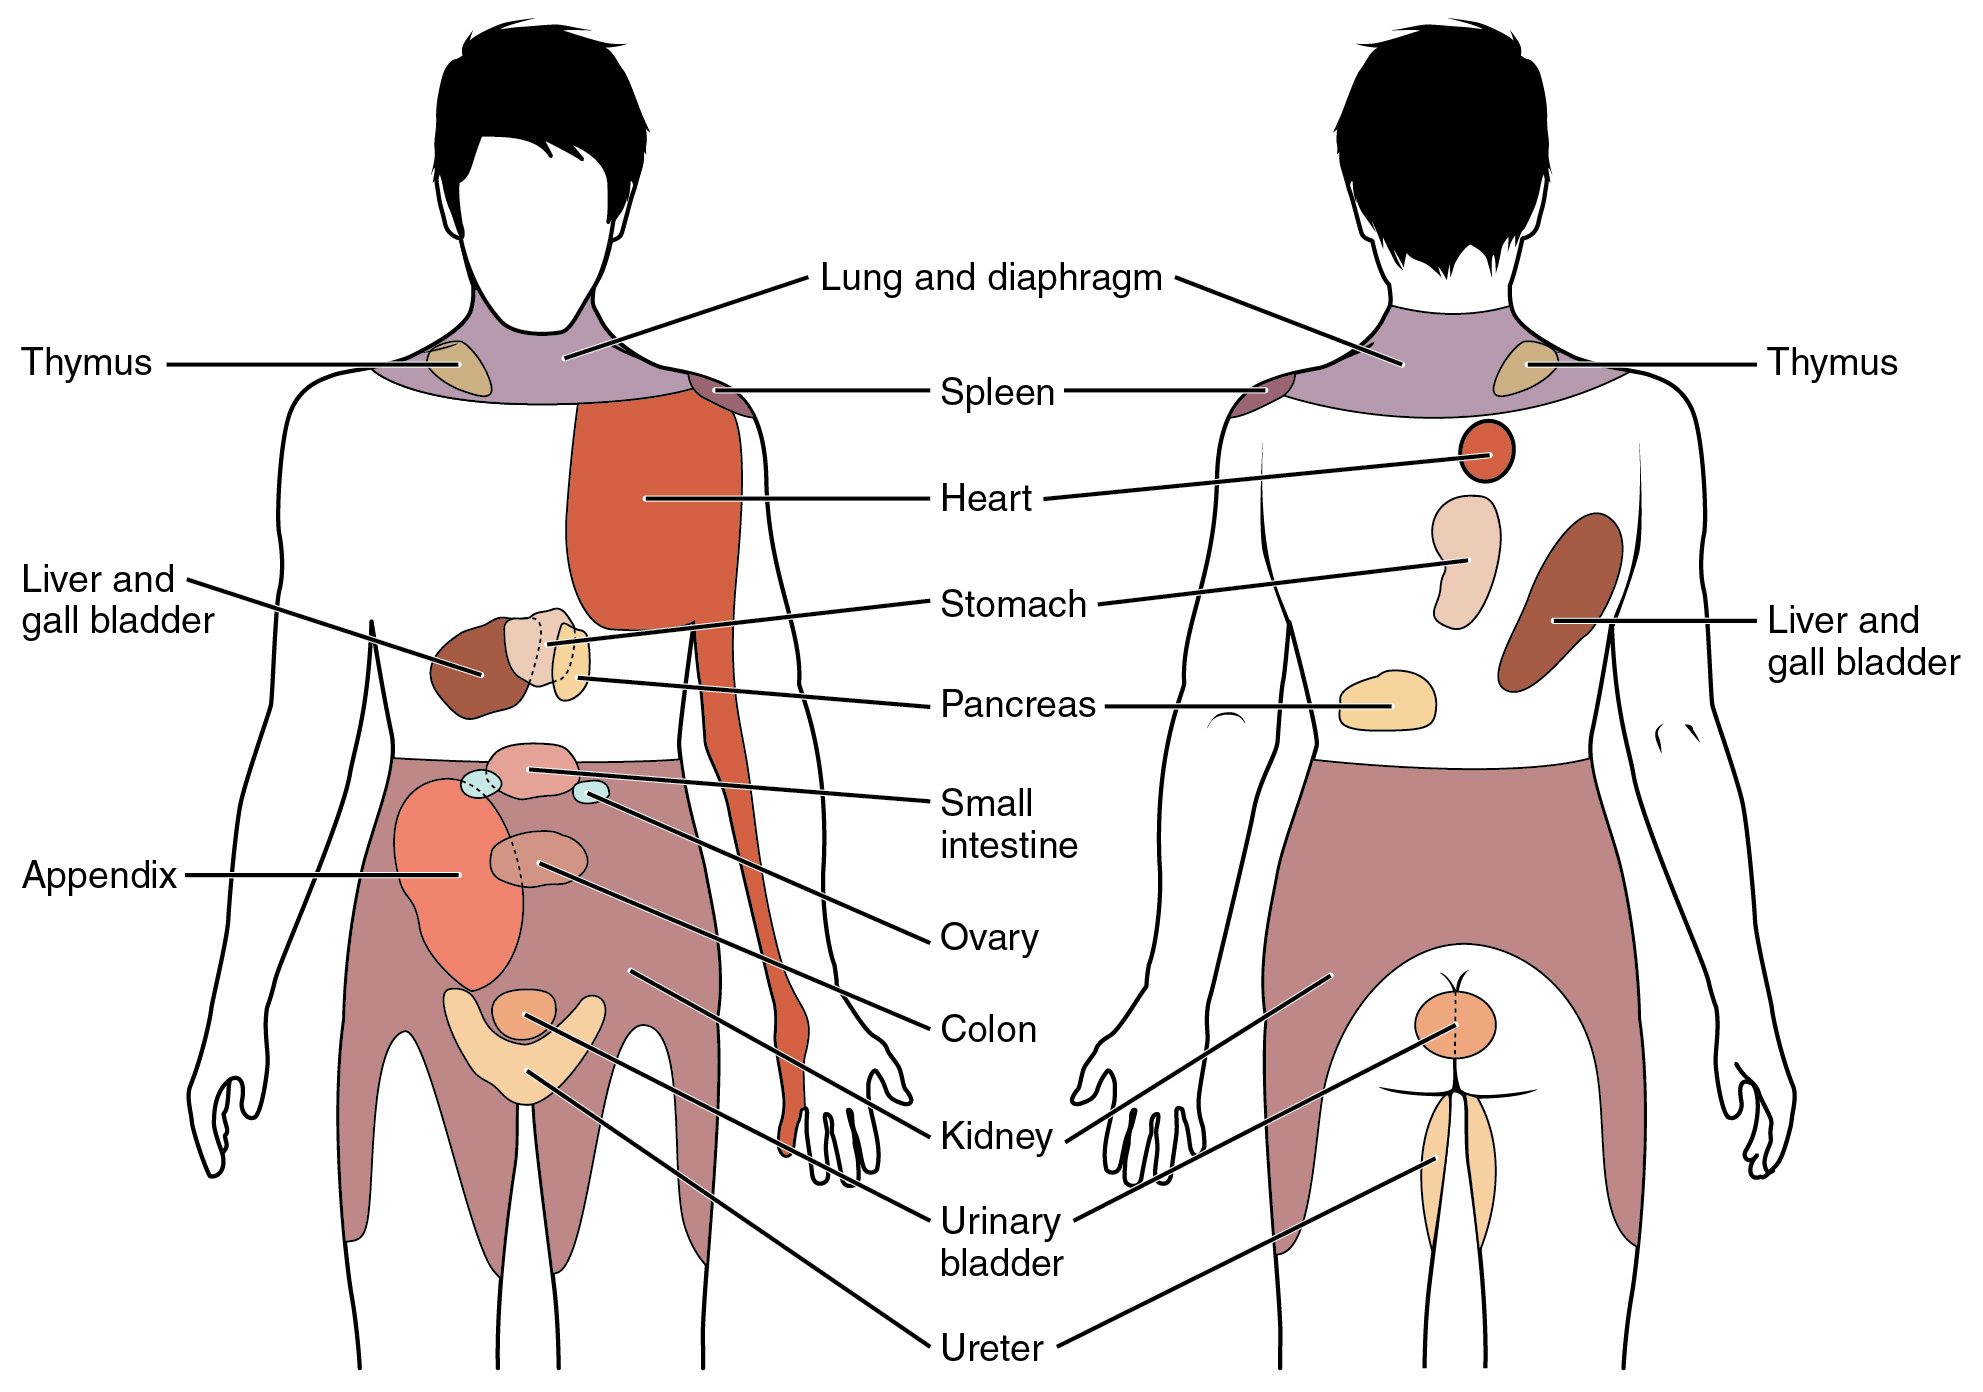
\includegraphics[width=0.7\textwidth]{Referred_Pain_Chart.jpg}
\end{center}

\end{frame}

\begin{frame}
\frametitle{Übertragener Schmerz}

OK \dots Aber warum? 


\pause

Mögliche Erklärung: Konvergenz im Rückenmark: Schmerzfasern aus den Viszera und aus den entsprechenden Haut-Regionen schalten im Rückenmark auf dieselben weiterleitenden Nervenfasern um. \\


\begin{center}
\includegraphics[width=\textwidth]{Schmerz_aufsteigend_bis_Rueckenmark.png}
\end{center}



\end{frame}


%% Schmerz aus dem Gesicht
\begin{frame}{Schmerz aus dem Gesicht}

Schmerz aus dem Gesicht geht nicht ins Rückenmark, sondern über das Ganglion trigeminale direkt in den Hirnstamm \\[0.2 cm]

\begin{center}
    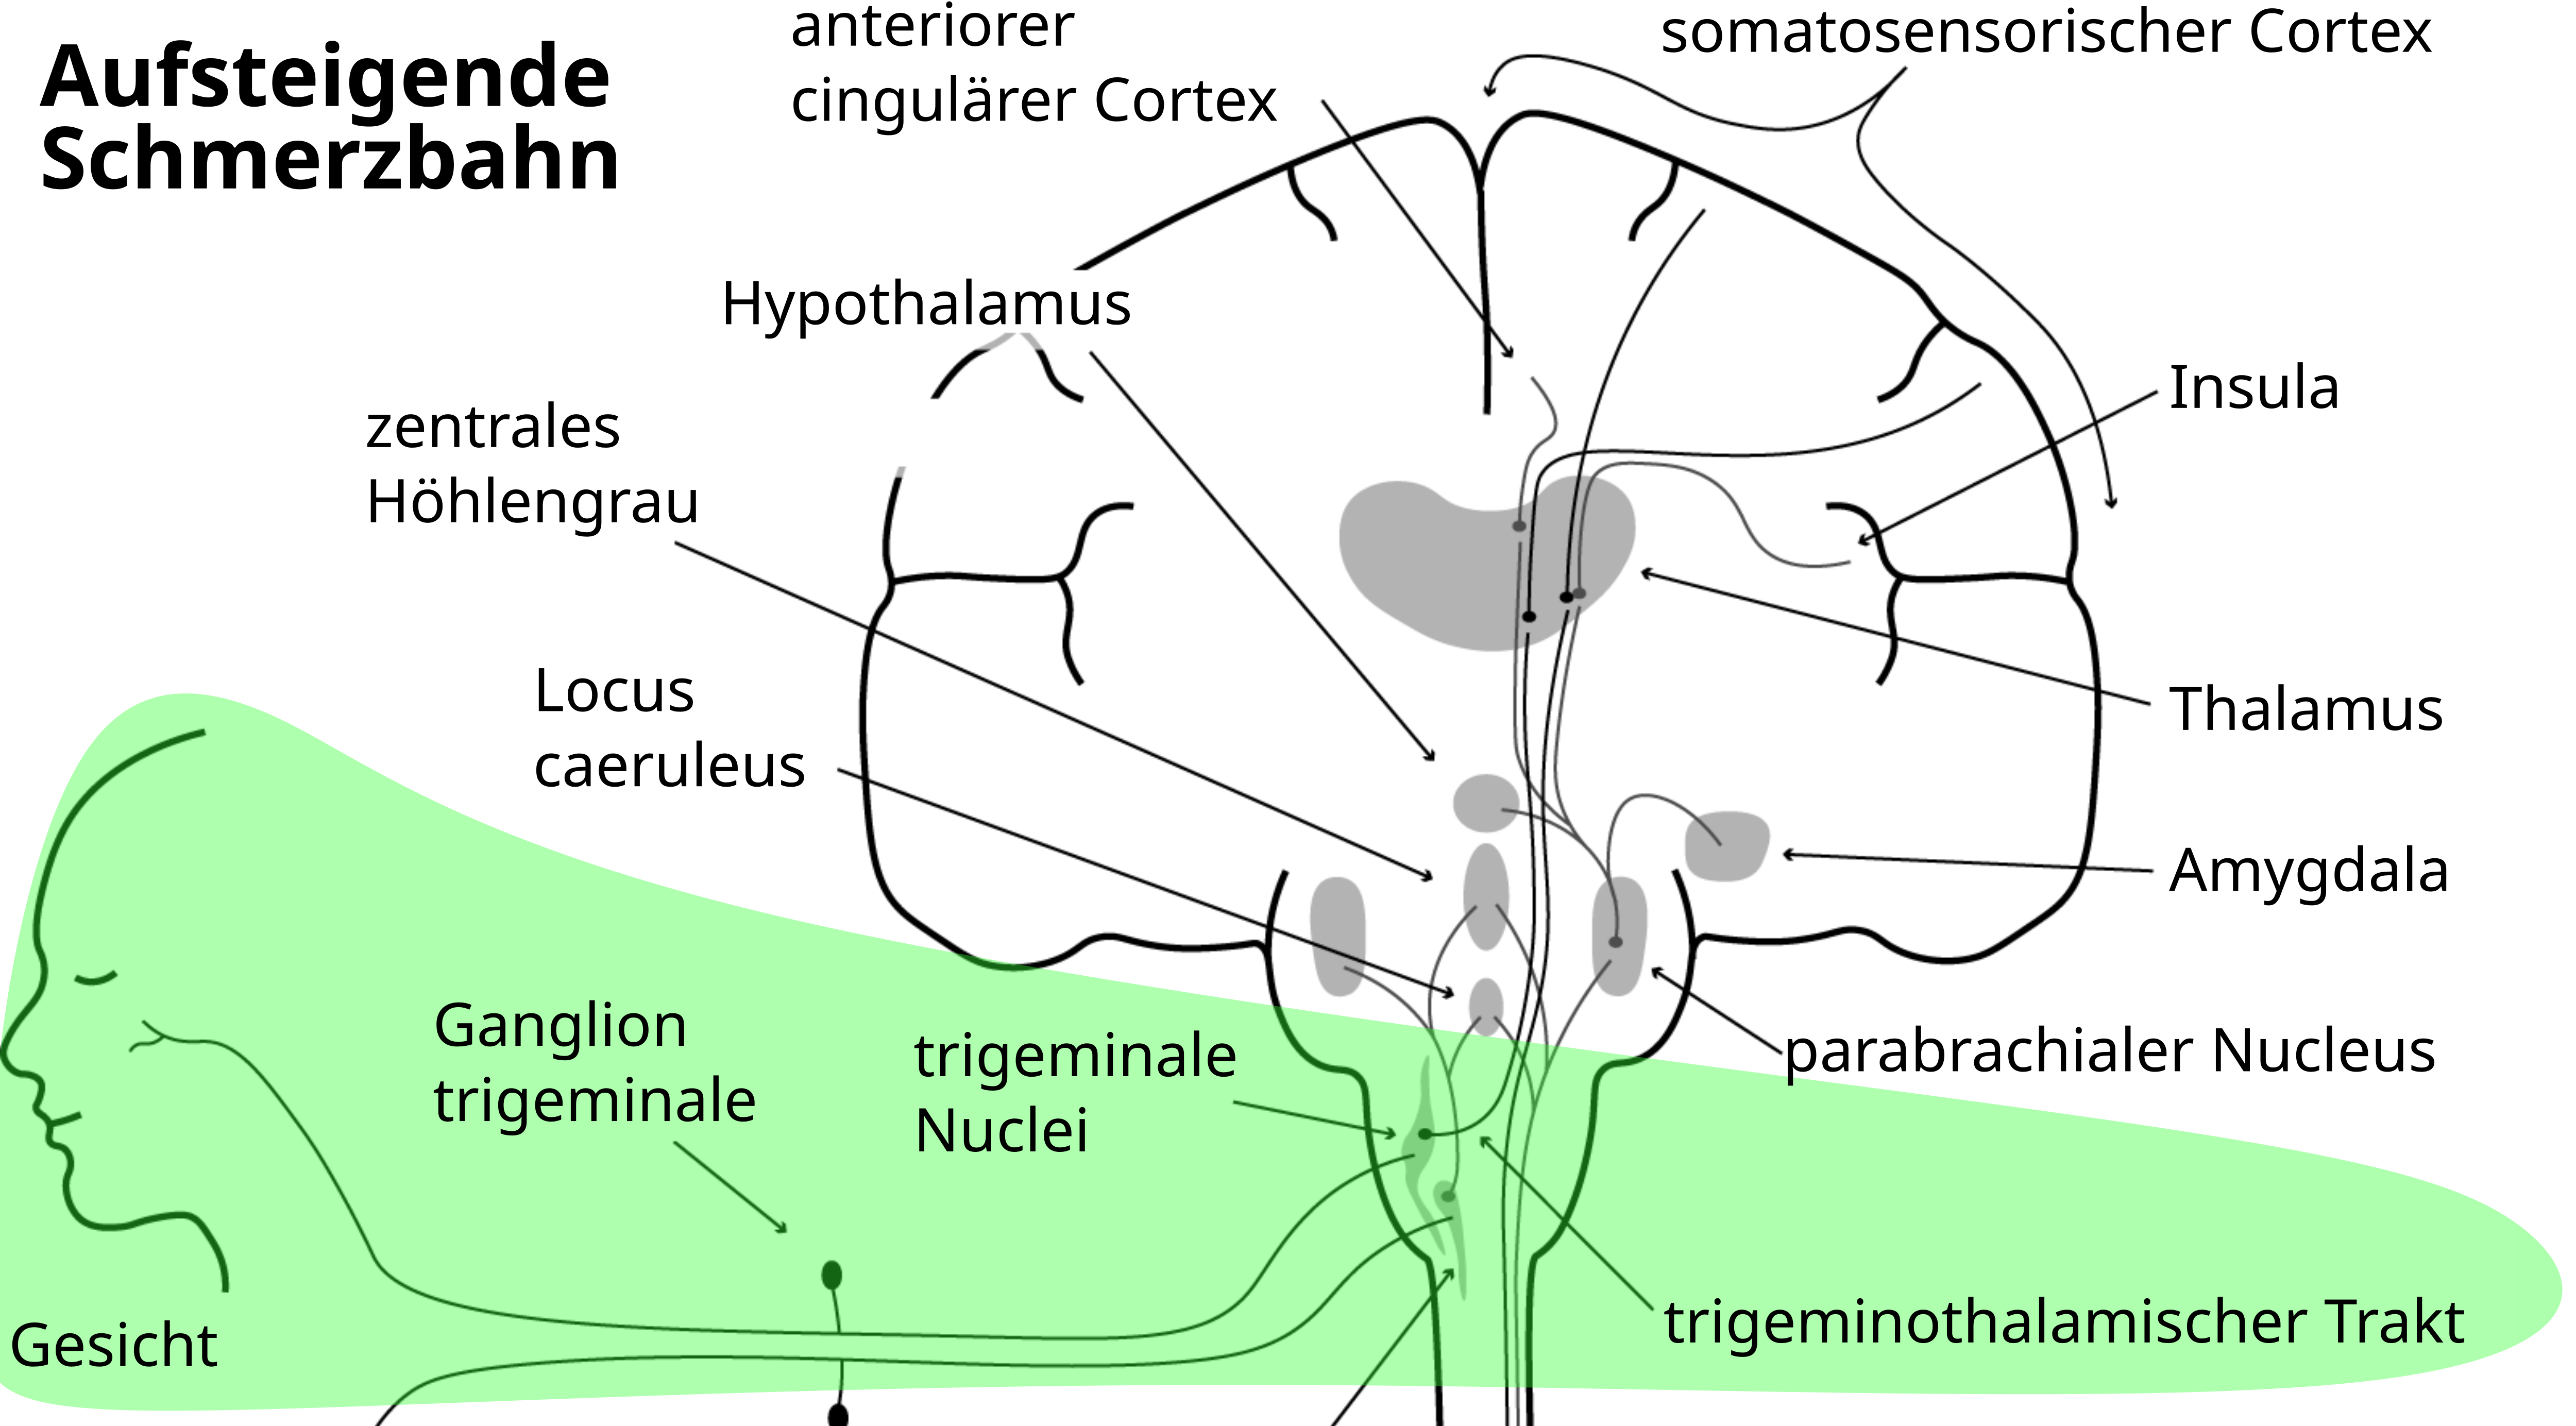
\includegraphics[width=0.9\textwidth]{Schmerz_aufsteigend_Gesicht.png}
\end{center}


\end{frame}





%%%%%%%%%%%%%%%%%%%%%%%%%%%%%%%%%%%%%%%%
%% Sensorische Zentren im Gehirn, Sinneseindruck, Wahrnehmung
%%%%%%%%%%%%%%%%%%%%%%%%%%%%%%%%%%%%%%%%

%% Übersicht 
\begin{frame}{Wahrnehmungsbahn}
    
    \begin{center}
        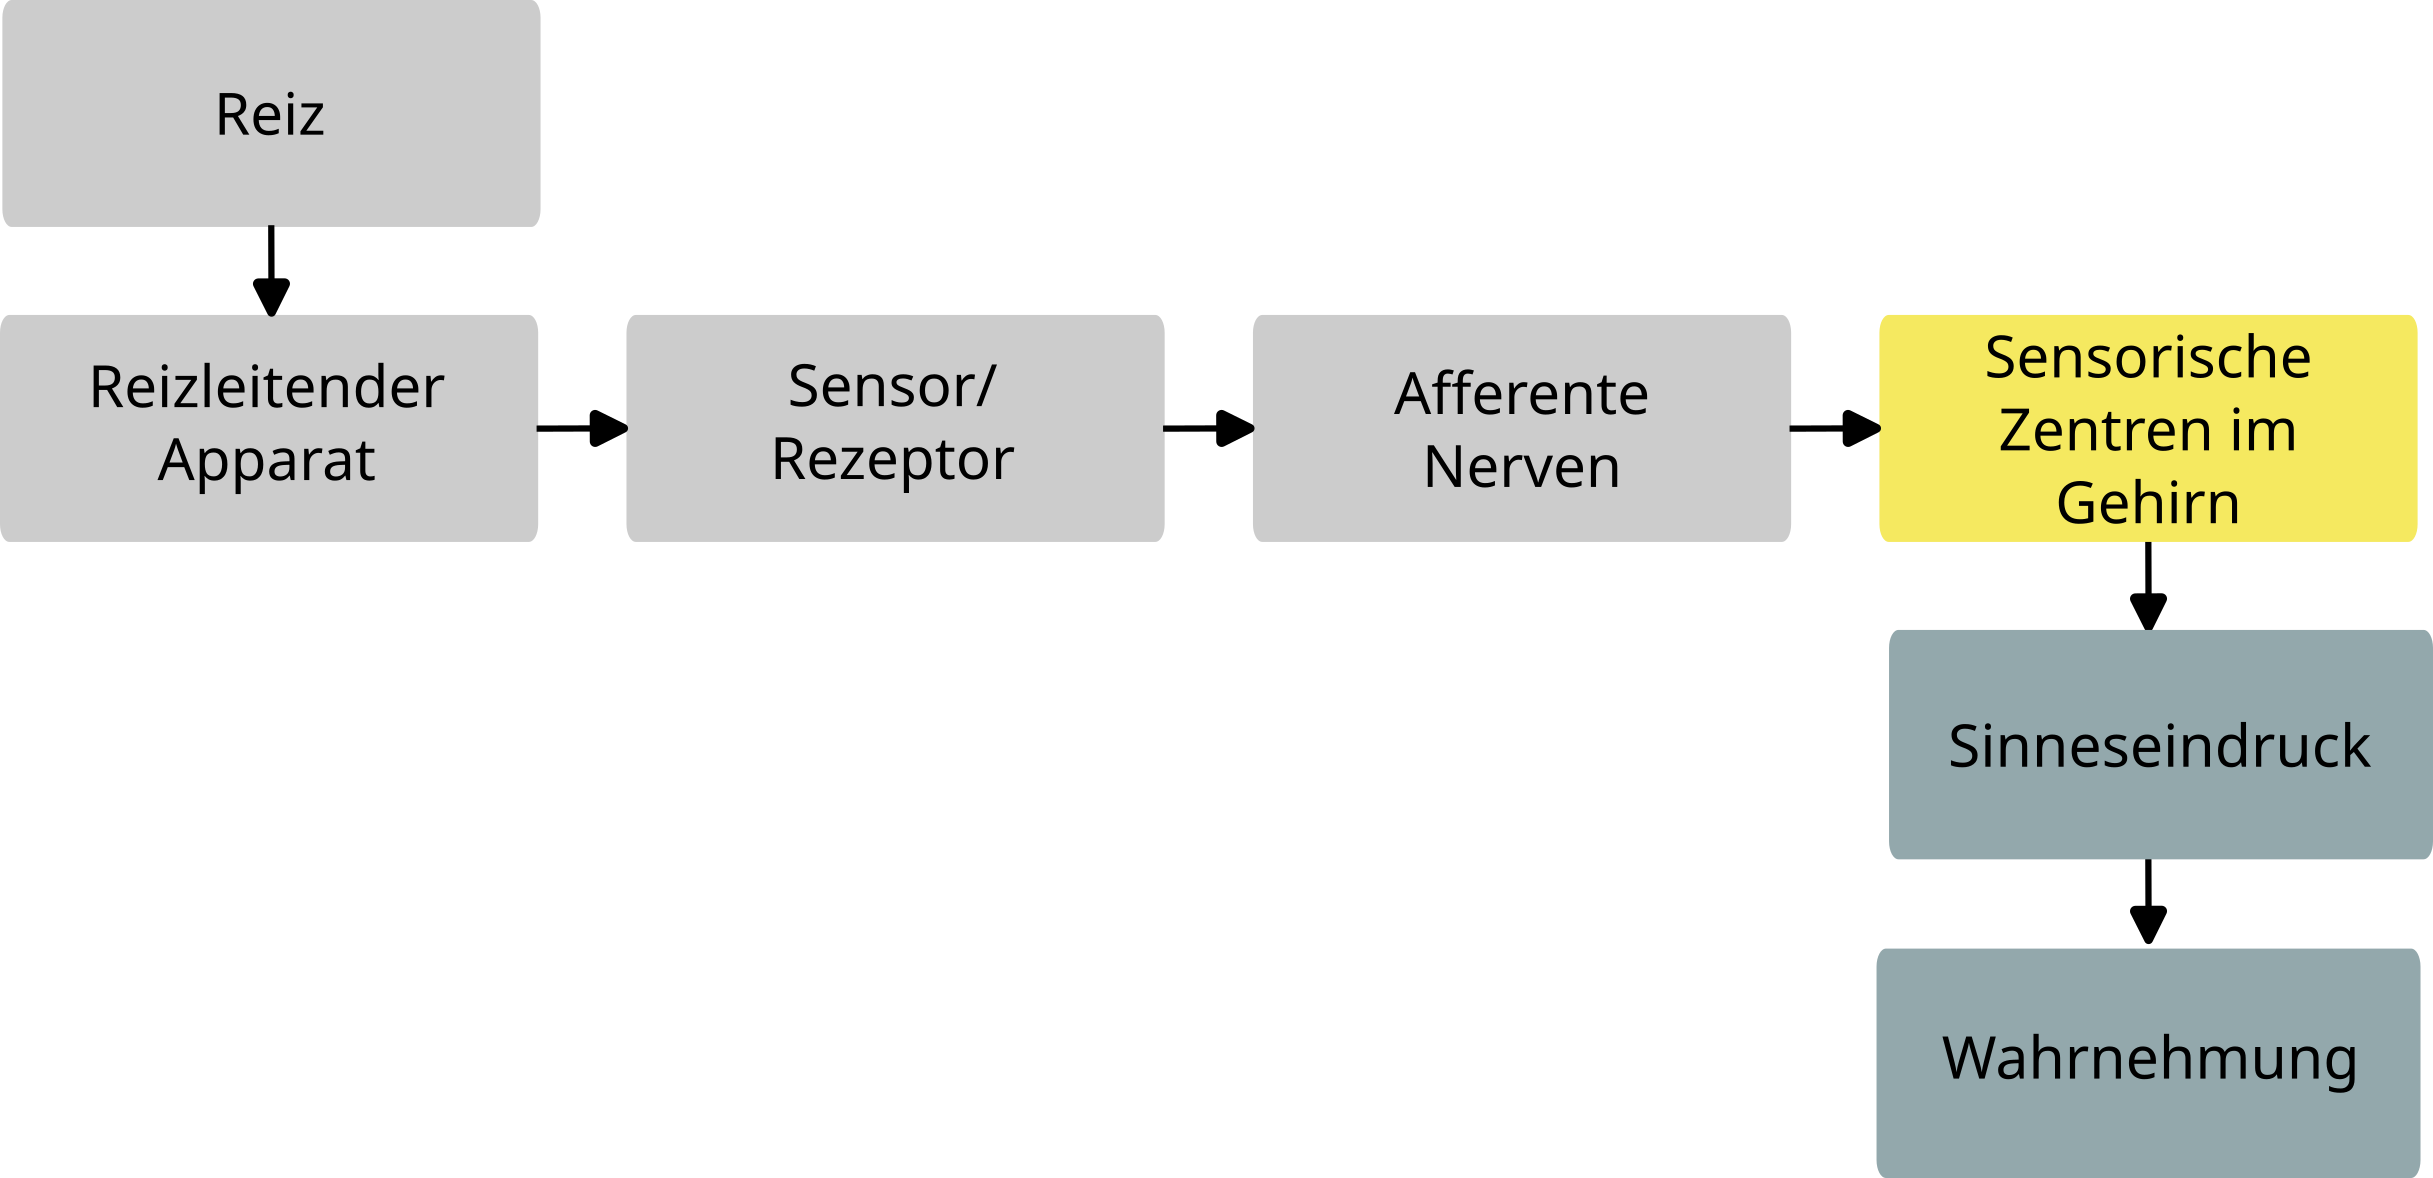
\includegraphics[width=\textwidth]{wahrnehmungsprozess_ohne_beispiel_gehirn.png}
    
    \end{center}
    
\end{frame}



%% Großes Schmerzbahn Bild

\begin{frame}{Gehirnregionen für Schmerzwahrnehmung}
    
    \begin{center}
        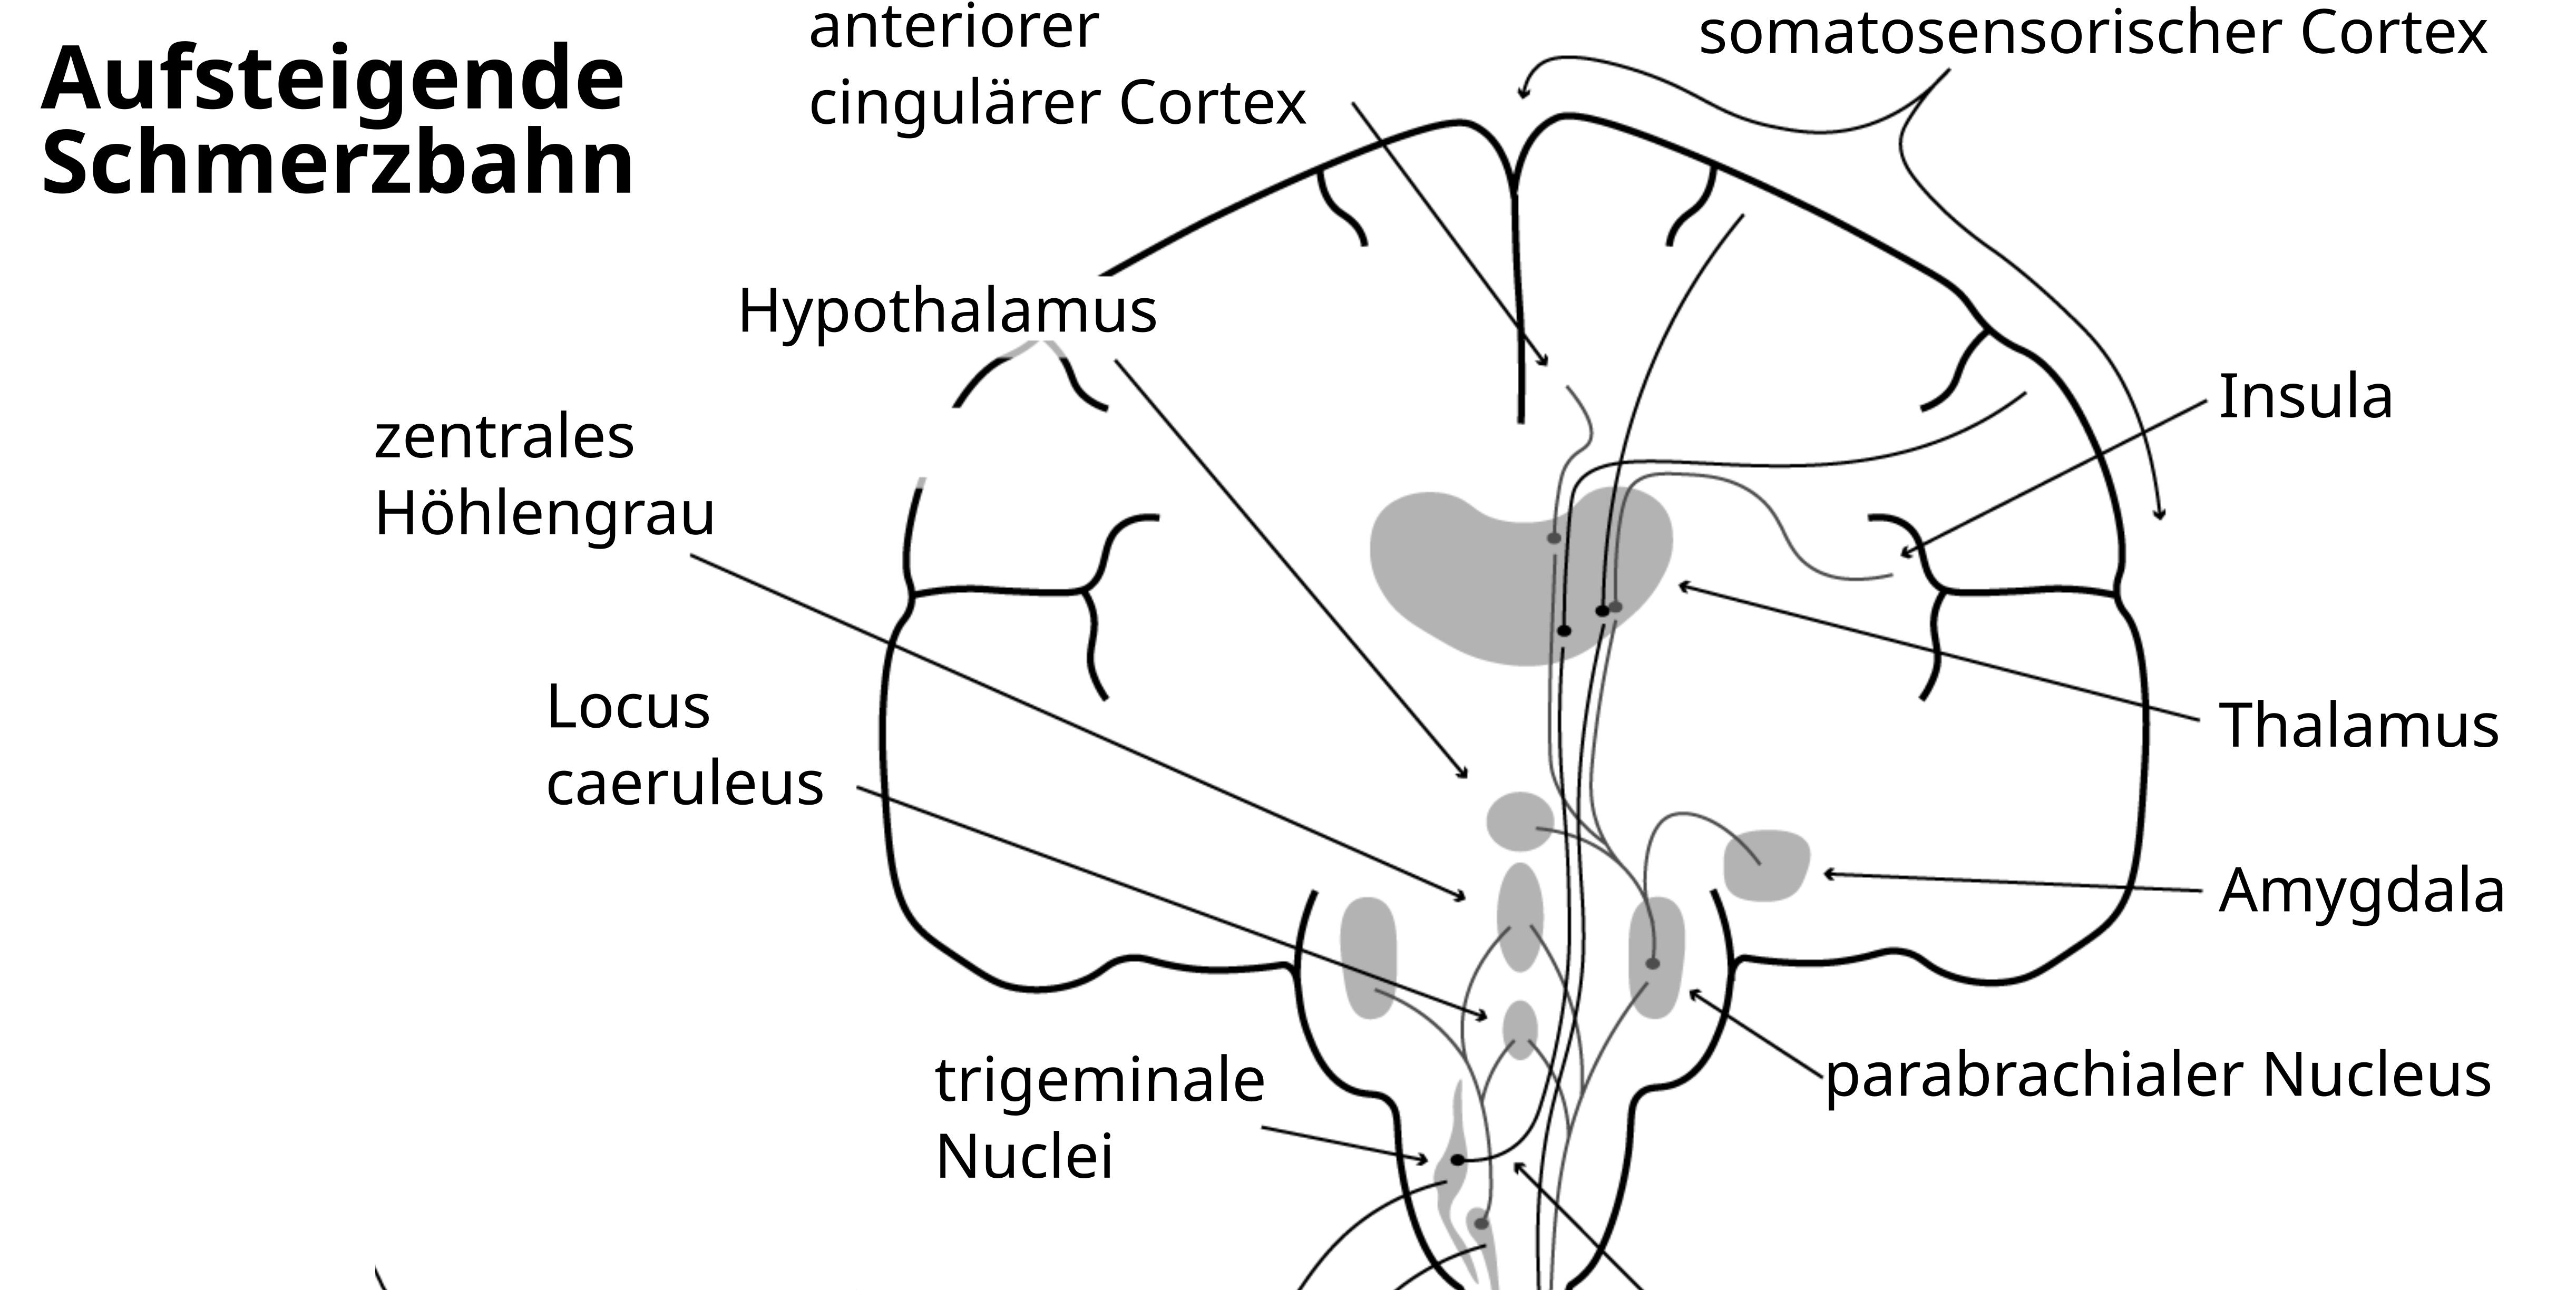
\includegraphics[width=\textwidth]{Schmerz_aufsteigend_Gehirn.png}
    
    \end{center}
    
\end{frame}


%% Thalamokortikales System
\begin{frame}{Thalamokortikales System}
    
    \begin{itemize}
        \item 
        Laterales System: Sensorisch-diskriminative Schmerzkomponente
        \item
        Mediales System: Affektive Schmerzkomponente
    \end{itemize}
    
    
\end{frame}

%% laterales System 
\begin{frame}{Laterales System}
    
    \begin{columns}[c]
    
    \begin{column}{5cm}
\begin{itemize}
\item
sensorisch-diskriminative Komponente
    \item Ventrolateralkomplex des Thalamus, Sensorische Cortexareale S1 und S2
    \item
    Erkennung, Lokalisierung und Klassifikation des Schmerzes
\end{itemize}
    
    \end{column}


    \begin{column}{5cm}
  %%%% Bild: Cerebrum
\begin{center}
    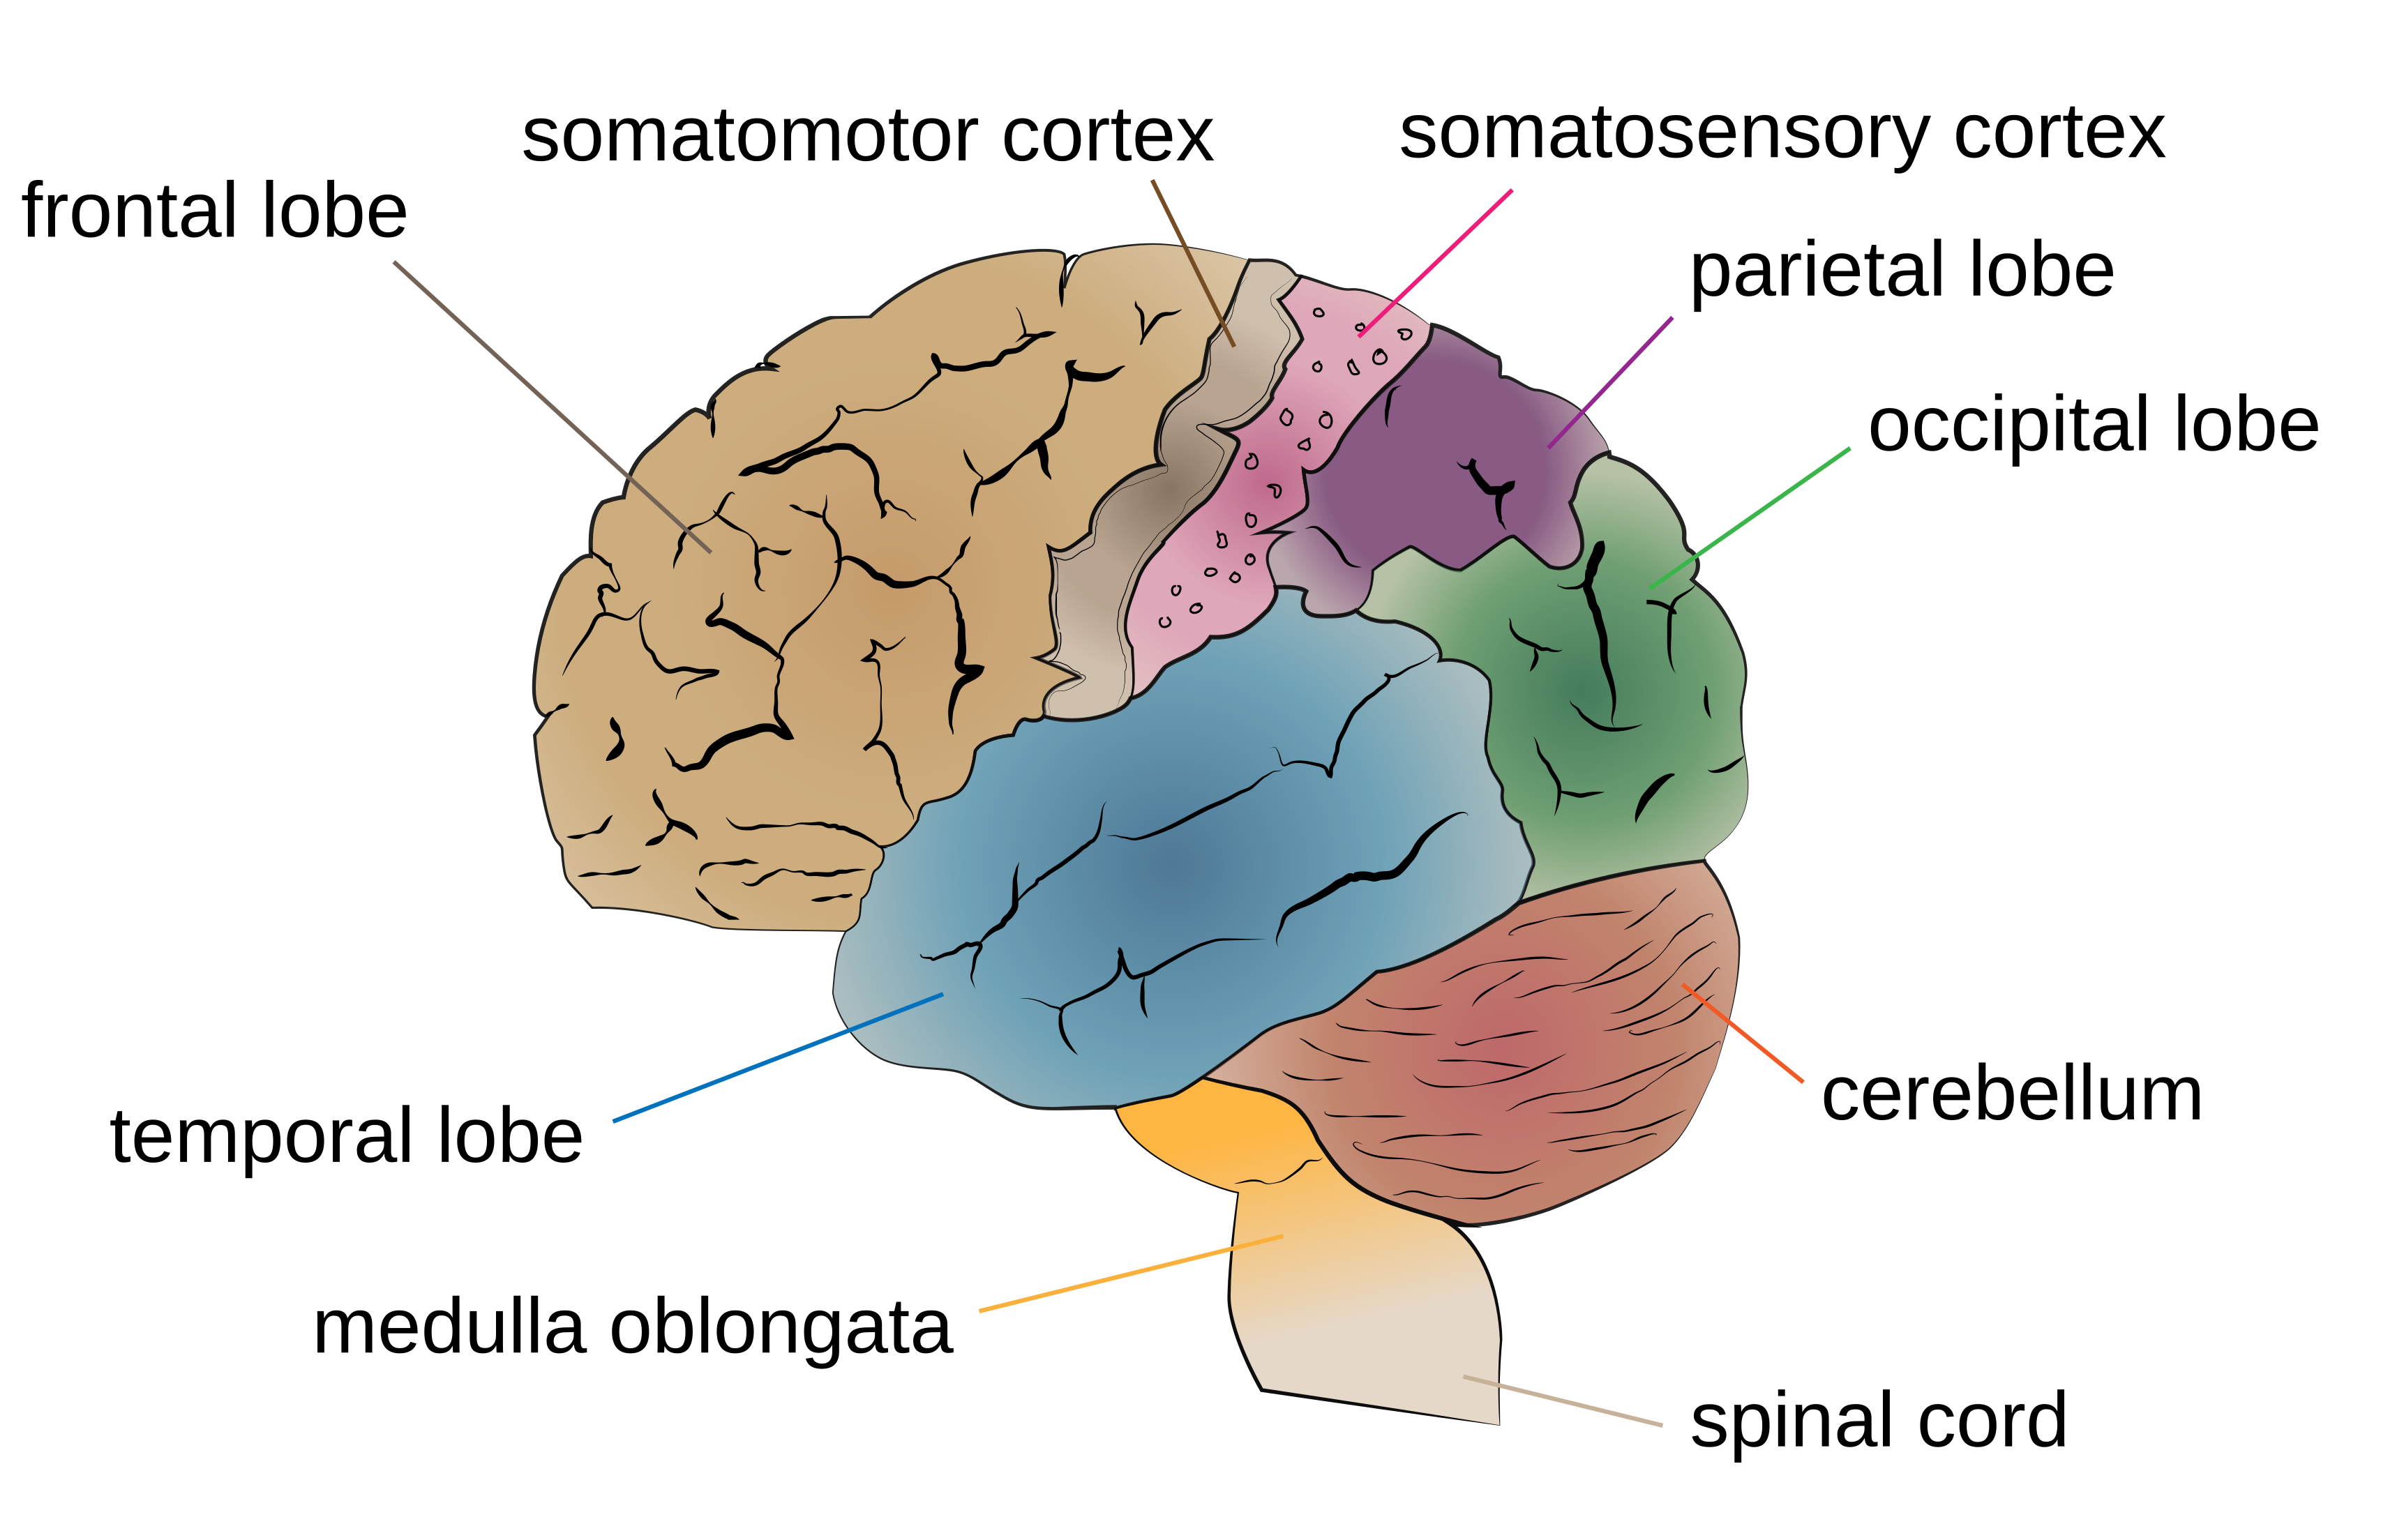
\includegraphics[width=\textwidth]{Cerebrum_lobes.png}
\end{center}    
    \end{column}
    
    \end{columns}
    
  
    
\end{frame}



\begin{frame}{Mediales System}
    
\begin{itemize}
\item
affektive Schmerzkomponente
\item
Posteriorer Komplex, interlaminären Komplexkerne des Thalamus, Verbindungen zu 
\begin{itemize}
    \item 
    Insula: Kommunikation mit dem limbischen System, Leiden
    \item
Gyrus cinguli anterior: Aufmerksamkeit, Antwortselektion
\item
präfrontaler Cortex: Entscheiden, Emotion, Persönlichkeit
\end{itemize}


\end{itemize}
    

    
\end{frame}



%% Mediales System

%% ARAS 
\begin{frame}{Im Schlaf spüren wir keinen Schmerz}

\begin{columns}[c]

\begin{column}{5cm}
\begin{center}
    
\includegraphics[width=\textwidth]{mathias-reding-4_YakZekVv0-unsplash.jpg}
\end{center}
\end{column}

\begin{column}{5cm}

Stimmt das? \\[0.5cm]
\pause

%% begin spoiler
Ja, denn Nozizeptoren und Neuronen der Schmerzbahn im Rückenmark können zwar aktiviert werden, aber es findet keine Schmerzverarbeitung im Thalamus statt.  \\[0.5cm]

\pause
Aber: Das ARAS erhält Eingänge aus dem Tractus spinothalamicus und dem Tractus spinalis nervi trigemini. Bei starken Schmerzreizen wird es aktiviert und führt zum Aufwachen. 

%% end spoiler
\end{column}


\end{columns}

    
\end{frame}

%% Amygdala
\begin{frame}{Amygdala}
    
    \begin{columns}[c]
    
    \begin{column}{6cm}
    
    \begin{center}
        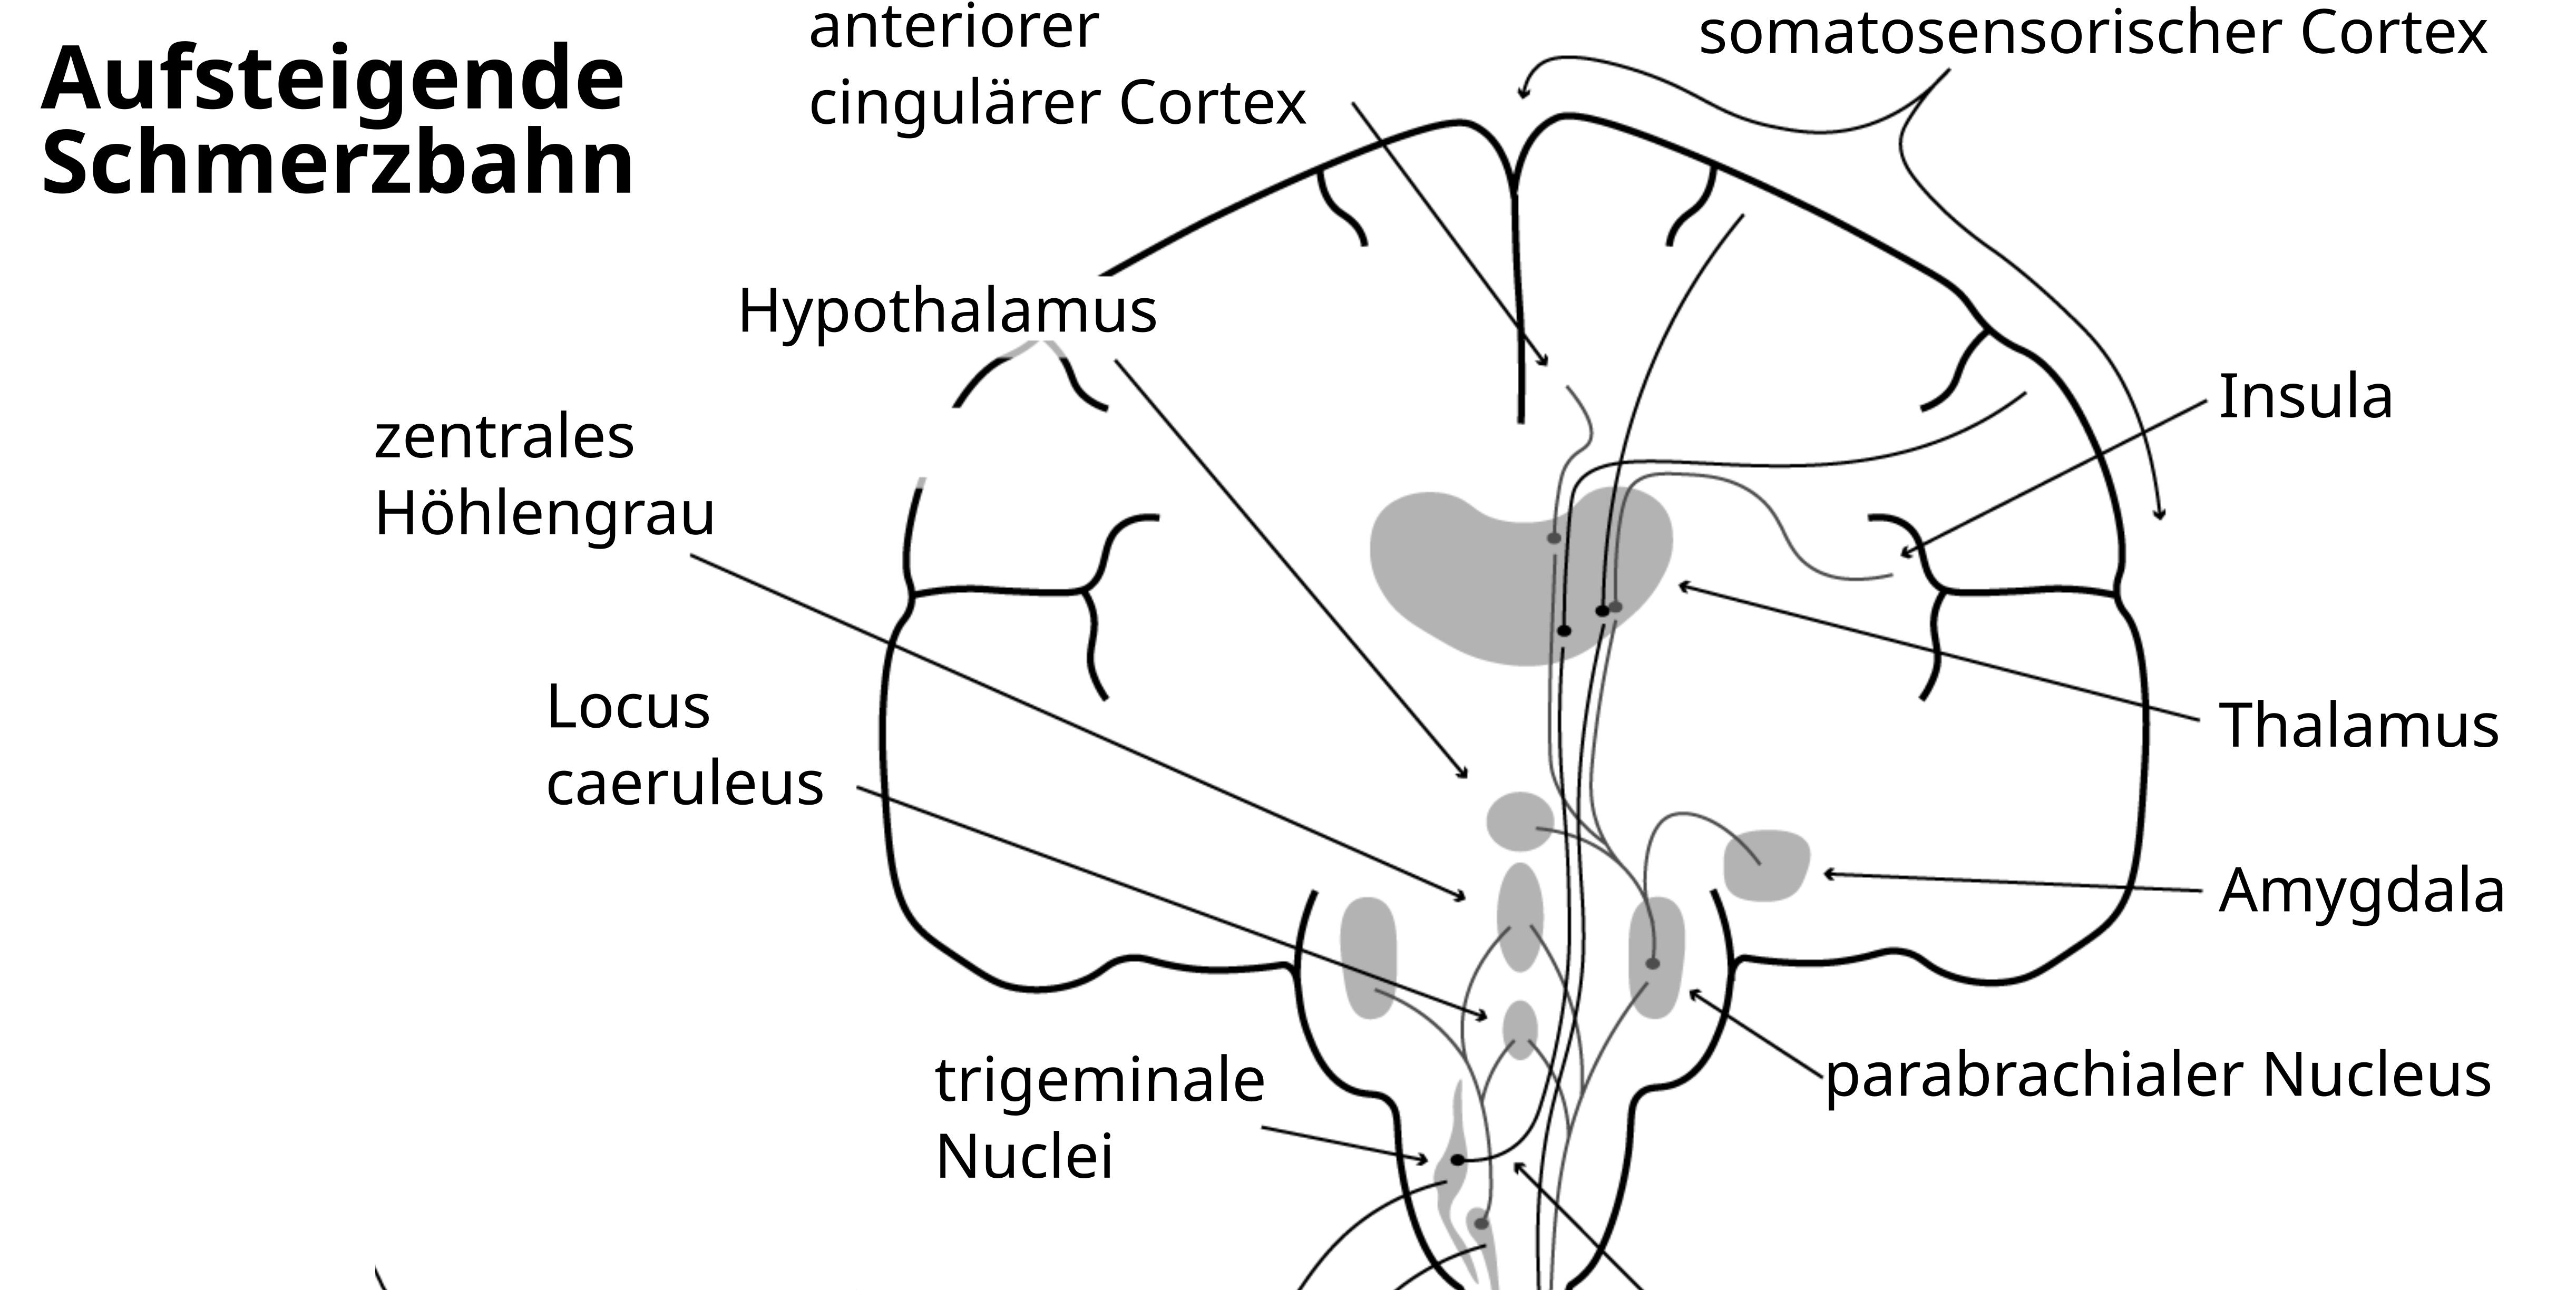
\includegraphics[width=\textwidth]{Schmerz_aufsteigend_Gehirn.png}
    
    \end{center}
    
    \end{column}

    \begin{column}{5cm}

Das nozizeptive System kommuniziert über die Amygdala mit dem Limbischen System  \\ [0.5 cm]

\(\rightarrow\) \pause Angst, Verbindung zwischen Schmerz und Depression


    
    \end{column}

    
    \end{columns}
    
\end{frame}





%% Absteigende Bahnen


\begin{frame}{Absteigende Bahnen}


\begin{columns}[c]

\begin{column}{7cm}
\begin{itemize}
    \item 
    Absteigende Bahnen aus dem Hirnstamm ins Rückenmark modifizieren die Schmerzwahrnehmung
    \item
    Beteiligt sind der Locus caeruleus und das zentrale Höhlengrau (über den Nucleus Raphe Magnus)
    \item
    Hemmung der Schmerzleitung durch GABA, Glycin und körpereigene Opioide (z.B. Metenkephalin)
    \item
    Verstärkung der Schmerzleitung durch Neuropeptide
\end{itemize}

\end{column}

\begin{column}{3cm}
\begin{center}
    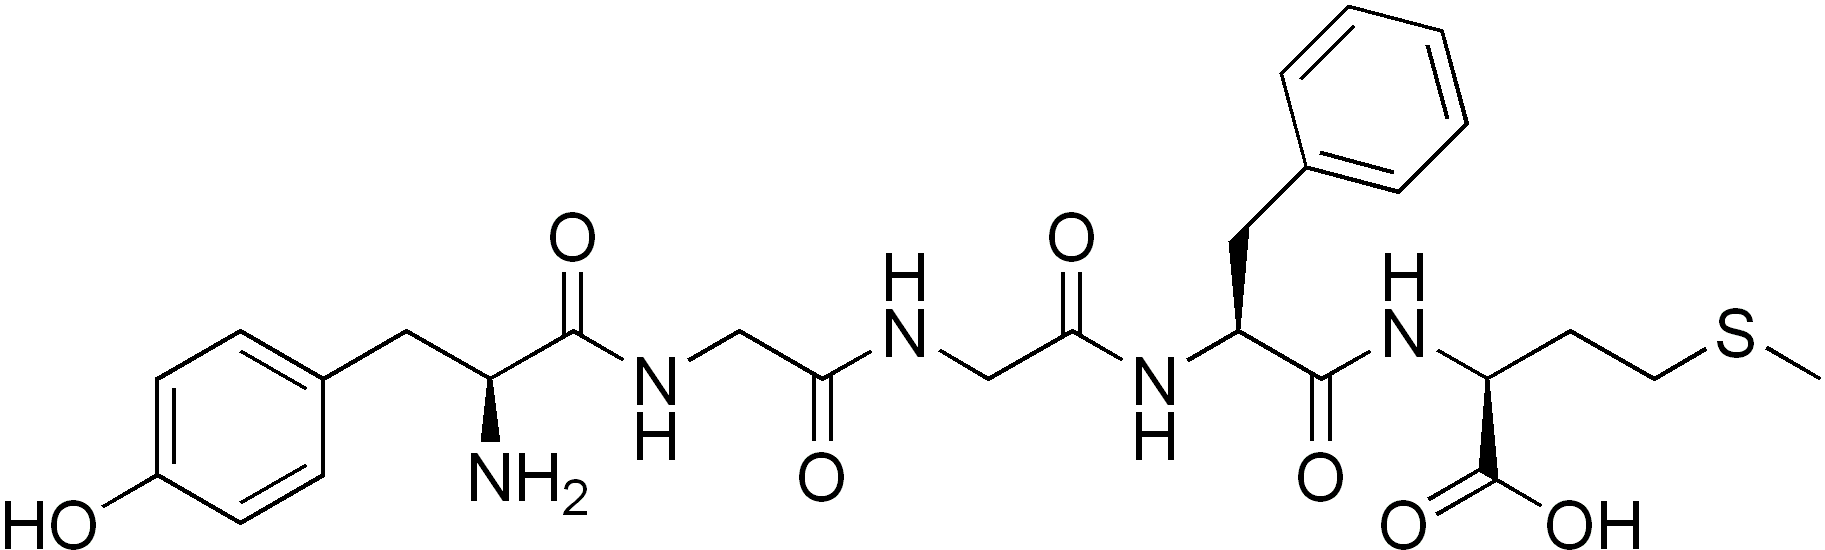
\includegraphics[width=2\textwidth, angle=90]{Met-enkephalin.png}
\end{center}
\end{column}


\end{columns}



\end{frame}


% \begin{frame}{Körpereigene Opioide}
% \begin{itemize}
%     \item Endorphine, Enkephaline, Dynorphine 
% \item Verschiedene Rezeptorklassen (\(\mu\), \(\delta\), \(\kappa\) ) sind relativ, aber nicht komplett selektiv für bestimmte Opioid-Klassen
% \item
% Alle Rezeptoren sind G-Protein gekoppelte Rezeptoren vom Typ G\textsubscript{S}
% \item
% Das heißt: \pause Sie hemmen Adenylatzyklase

% \end{itemize}

% \end{frame}






%%%% IMPP Frage

\begin{frame}{IMPP Frage}


Ein 60-jähriger Patient hat u.a. Schmerzen in der linken Schulter, die in den linken Arm ausstrahlen. Ein EKG bestätigt den Verdacht auf einen Herzinfarkt. Dieses Schmerzphänomen im linken Arm bei einem Myokardinfarkt wird (von den angegebenen Begriffen) am besten bezeichnet als 

\begin{description}
    \item[A.] emotionale Schmerzkomponente
    \item[B.] kognitive Schmerzkomponente
    \item[C.] neuropathischer Schmerz
    \item[D.] Phantomschmerz
    \item[E.] übertragener Schmerz
\end{description}
    
\end{frame}


%% Spoiler Alert
\begin{frame}
\frametitle{Erinnerung: Übertragener Schmerz/Head-Zonen}



\begin{center}
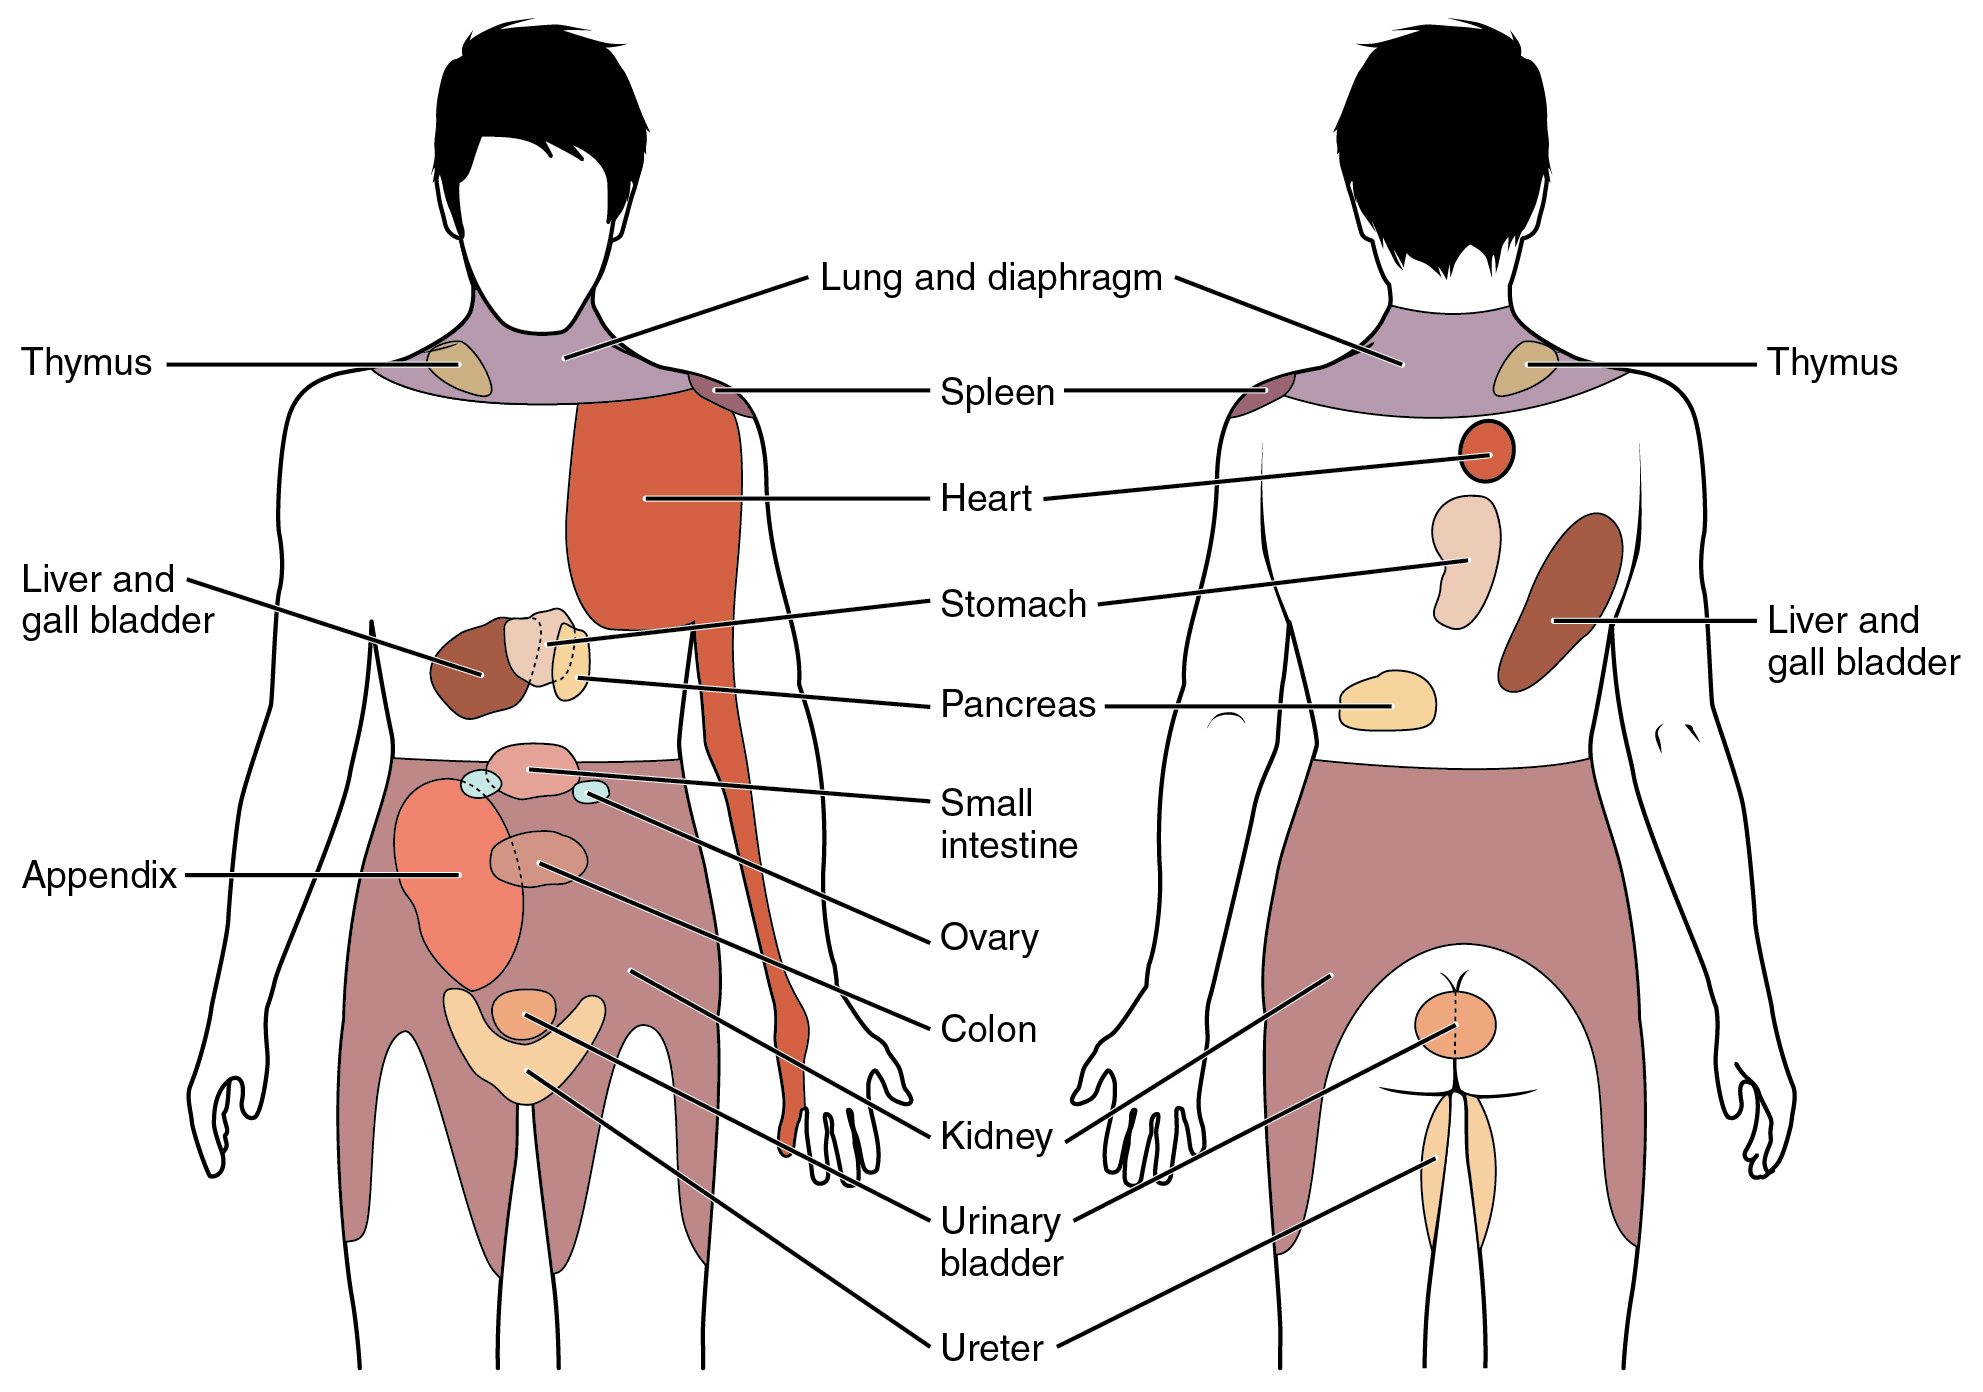
\includegraphics[width=0.9\textwidth]{Referred_Pain_Chart.jpg}
\end{center}

\end{frame}
%%  End Spoiler Alert



%% Review

\begin{frame}


 \frametitle{Jetzt* sollten Sie folgendes können}



\begin{block}{Grundlagen:}




\begin{itemize}

    \item 
    
Arten von Nozizeptoren beschreiben und erklären
    \item 
 schnellen und langsamen Schmerz unterscheiden und deren neurobiologische Grundlagen erläutern
    \item 
 endogene Mediatoren der Nozizeptorerregung benennen und erläutern
    \item 
    Hyperalgesie und Allodynie definieren
    \item 
 Neuropeptide beschreiben, die aus Nozizeptoren freigesetzt werden und deren Wirkung erläutern
    \item 
 neurogene Vasodilatation und Entzündung erläutern
    \item 
 Aufsteigende Schmerzbahnen beschreiben
    \item 
 die Schmerzübertragung bei viszeraler Nozizeption erklären
    \item 
erklären, welche  Hirnregionen an der Schmerzempfindung teilhaben
    \item 
 projizierten Schmerz definieren

\end{itemize}


\end{block}

\end{frame}


\begin{frame}


 \frametitle{Jetzt* sollten Sie folgendes können}
 

\begin{block}{Klinik:}

\begin{itemize}
    
\item 
Schmerztherapien aufzählen und erklären
    \item 
     Phantomschmerzen definieren
    \item 
 Beispiele für Krankheiten mit erhöhtem und vermindertem Schmerzempfinden geben. 
\item
Head-Zonen beschreiben

\end{itemize}


\end{block}


$\,$\\[1cm]
\textcolor{theme}{Welche Fragen haben Sie?}


\end{frame}


%% %% %% %% Feedbackhinweisblock

\begin{frame}
\frametitle{Danke für Ihr Feedback!}

\begin{columns}[c]

\begin{column}{6cm}
\begin{center}
 
\includegraphics[width=\textwidth]{smilie_balloons.jpg}
\end{center}

\end{column}

\begin{column}{4cm}


\begin{center}

\includegraphics[width=\textwidth]{feedback_QR.png}
\end{center}
\end{column}


\end{columns}
\end{frame}




\begin{frame}
 
\frametitle{Bildnachweis}
 
\begin{tiny}
  

\begin{itemize}

\item
Chilischoten. Photo by K8 on Unsplash. 

\item
Gehirn mit Hervorhebung des somatosensorischen Cortex. By vectorized by Jkwchui - \url{http://training.seer.cancer.gov/module_anatomy/unit5_3_nerve_org1_cns.html}, CC BY-SA 3.0, \url{https://commons.wikimedia.org/w/index.php?curid=29055751}

\item
Head-Zonen. OpenStax College - Autonomic Reflexes and Homeostasis  \url{http://cnx.org/content/m46579/1.2/}, CC BY 3.0, \url{https://commons.wikimedia.org/w/index.php?curid=30017359}

\item
Innere Organe.  Sue Clark - Flickr: View of Viscera Page 82, Public Domain, \url{https://commons.wikimedia.org/w/index.php?curid=16128601}

\item
Ionenkanal.  Original uploader was Outslider (Paweł Tokarz) at pl.wikipedia - Transferred from pl.wikipedia to Commons by Masur using CommonsHelper., Public Domain, \url{https://commons.wikimedia.org/w/index.php?curid=5828577}
\item
Joe Thomas und Simone Biles. Erik Drost, CC BY 2.0 \url{https://creativecommons.org/licenses/by/2.0}, via Wikimedia Commons

\item
Kaktus. Photo by \href{https://unsplash.com/@earl_plannerzone?utm_source=unsplash&utm_medium=referral&utm_content=creditCopyText}{Earl Wilcox} on \href{https://unsplash.com/s/photos/pain?utm_source=unsplash&utm_medium=referral&utm_content=creditCopyText}{Unsplash}

\item
La Columna Rota. By Frida Kahlo/Museo Dolores Olmedo - \url{http://www.tate.org.uk/whats-on/tate-modern/exhibition/frida-kahlo/frida-kahlo-room-guide/frida-kahlo-room-guide-room-11}, Fair use, \url{https://en.wikipedia.org/w/index.php?curid=47997195}


\item
Luftballons mit frohen und traurigen Smileys. Photo by \href{https://unsplash.com/@artbyhybrid?utm_source=unsplash&utm_medium=referral&utm_content=creditCopyText}{Hybrid} on \href{https://unsplash.com/s/photos/feedback?utm_source=unsplash&utm_medium=referral&utm_content=creditCopyText}{Unsplash}

\item
Metenkephalin. Von Edgar181 - Eigenes Werk, Gemeinfrei, \url{https://commons.wikimedia.org/w/index.php?curid=2834218}

\item
Prostaglandin-Synthese. Eigenes Bild, 2021. CC BY-SA 3.0.

\item
Schlafende Katze. Photo by \href{https://unsplash.com/@matreding?utm_source=unsplash&utm_medium=referral&utm_content=creditCopyText}{Mathias Reding} on \href{https://unsplash.com/s/photos/sleep?utm_source=unsplash&utm_medium=referral&utm_content=creditCopyText}{Unsplash}
  

\item
Schmerzbahn (und Ausschnitte davon). Eigene Bilder, 2021, CC BY 4.0 \url{https://creativecommons.org/licenses/by/4.0} nach einem Bild von Richard Lennertz,  Wikimedia Commons

\item
Sonnenbrand. By Phil Kates - \url{https://www.flickr.com/photos/hawk684/108139247/}, CC BY-SA 2.0, \url{https://commons.wikimedia.org/w/index.php?curid=51031248}

\item
Substanz P. Fvasconcellos - Own work, Public Domain, \url{https://commons.wikimedia.org/w/index.php?curid=1017110}

\item
TRPV1. Von The Author 2011. Published by Oxford University Press - \url{https://www.ncbi.nlm.nih.gov/core/lw/2.0/html/tileshop_pmc/tileshop_pmc_inline.html?title=Click on image to zoom&p=PMC3&id=3169333_aer26002.jpg}
CC BY-SA 2.5, \url{https://commons.wikimedia.org/w/index.php?curid=34131563}

\item
Wahrnehmungsbahn und einzelne Prozesse entlang der Wahrnehmungsbahn (mehrere Bilder). Mein eigenes Werk, CC BY-SA 4.0, 2022. 

\item
Wirkung von nozizeptiven Neuropeptiden. Mein eigenes Werk, 2021. CC BY-SA 4.0. 

\end{itemize}
\end{tiny}

\end{frame}




%%%%%%%%%%%%%%%%%%%%%%%%%%%%%%%%%%%%%%%%%%%%%%
%%% Previous material
%%%%%%%%%%%%%%%%%%%%%%%%%%%%%%%%%%%%%%%%%%%%%%


% \begin{frame}
% \frametitle{Wie der Schmerz ins Rückenmark kommt}

% \pause 
% \begin{center}
% \includegraphics[width=\textwidth]{/home/melanie/Work/pictures/brain/Schmerz_aufsteigend_bis_Rueckenmark.png}
% \end{center}

% \end{frame}


% %% Learning Objectives
%  \begin{frame}
% \frametitle{Lernziele}


% \begin{block}{Nach dieser Vorlesung werden Sie folgendes können:}



% \begin{itemize}
% \item
% Den allgemeinen Weg des Schmerzreizes vom Nozizeptor bis ins Gehirn beschreiben
% \item
% Die drei Arten von Nozizeption aufzählen und beschreiben
% \item
% Erklären, wie Schmerz-Rezeptoren aktiviert werden
% \item
% Modifikatoren von Schmerz-Rezeptoren benennen und erklären
% \item
% Erklären, was schnellen von langsamem Schmerz unterscheidet
% \item
% Erklären, was  übertragener Schmerz ist und wann er vorkommt
% \end{itemize}


% \end{block}


% \end{frame}


% %% Main Body


% %% Überblick Schmerz ins Hirn
% \begin{frame}
% \frametitle{Wie der Schmerz ins Hirn kommt}

% \begin{center}
% \includegraphics[width=0.5\textwidth]{/home/melanie/Work/pictures/brain/Schmerz_aufsteigend.png}
% \end{center}

% \end{frame}








%   %% Big picture Überblick
% \begin{frame}
% \frametitle{Zusammenfassung}

% \begin{center}
% \includegraphics[width=\textwidth]{/home/melanie/Work/pictures/brain/Schmerz_aufsteigend_bis_Rueckenmark.png}
% \end{center}

% \end{frame}







% \begin{frame}
% \frametitle{Welche der Fragen vom Anfang haben wir beantwortet?}

% \begin{itemize}
% \item
% Warum ist auf Sonnenbrand alles schmerzhaft, sogar ein T-Shirt?
% \item
% Wie funktioniert eigentlich Aspirin? 
% \item
% Warum können Schmerzen im Arm ein Anzeichen von Herzinfarkt sein? 
% \item
% Warum kann man bei Schmerzen schlecht schlafen? 
% \item
% Warum tut es weh, besonders scharfe Chilis zu essen?
% \item
% Warum haben manche Menschen nie Schmerzen? Und andere dauernd?
% \item
% Warum hilft Bewegung bei Regelschmerzen? 
% \item
% Wie funktionieren Phantomschmerzen?  
% \item
% \dots 
% \end{itemize}

% \end{frame}



% %% Auflösung: Beantwortete Fragen
% \begin{frame}
% \frametitle{Welche der Fragen vom Anfang haben wir beantwortet?}

% \begin{itemize}
% \item
% \textcolor{theme}{Warum ist auf Sonnenbrand alles schmerzhaft, sogar ein T-Shirt?}
% \item
% \textcolor{theme}{Wie funktioniert eigentlich Aspirin?} 
% \item
% \textcolor{theme}{Warum können Schmerzen im Arm ein Anzeichen von Herzinfarkt sein?}
% \item
% Warum kann man bei Schmerzen schlecht schlafen? 
% \item
% \textcolor{theme}{Warum tut es weh, besonders scharfe Chilis zu essen?}
% \item
% Warum haben manche Menschen nie Schmerzen? Und andere dauernd?
% \item
% \textcolor{theme}{Warum hilft Bewegung bei Regelschmerzen?} 
% \item
% Wie funktionieren Phantomschmerzen?  
% \item
% \dots 
% \end{itemize}

% \end{frame}



% %% Review
%  \begin{frame}
% \frametitle{Lernziel-Check}


% \begin{block}{Jetzt sollten Sie folgendes können:}



% \begin{itemize}
% \item
% Den allgemeinen Weg des Schmerzreizes vom Nozizeptor bis ins Gehirn beschreiben
% \item
% Die drei Arten von Nozizeption aufzählen und beschreiben
% \item
% Erklären, wie Schmerz-Rezeptoren aktiviert werden
% \item
% Modifikatoren von Schmerz-Rezeptoren benennen und erklären
% \item
% Erklären, was schnellen von langsamem Schmerz unterscheidet
% \item
% Erklären, was übertragener Schmerz ist und wann er vorkommt
% \end{itemize}


% \end{block}

% \pause

% Welche Fragen haben Sie? 

% \end{frame}








\end{document}




